\documentclass[dvips,landscape]{foils}
\usepackage{graphicx}
\usepackage{graphics}
\usepackage{amsmath}
\usepackage{amsthm}
\usepackage[all]{xy}
\usepackage{amsfonts}
\input defs.tex
\raggedright
\special{! TeXDict begin /landplus90{true}store end }
\renewcommand{\oursection}[1]{
\foilhead[-1.0cm]{#1}
}

\graphicspath{{figures/}}

\title{Cutoffs in Chaotic Map Mixing and Topology Optimization of Microfluidic Channels}
\author{Tzu-Chen Liang}
\MyLogo{Tzu-Chen Liang, Stanford University}
\date{\today}
\newtheorem{definition}{Definition}
\newtheorem{example}{Example}
\newtheorem{theorem}{Theorem}
\newtheorem{lemma}{Lemma}
\DeclareMathOperator{\erf}{erf}
\DeclareMathOperator{\prob}{\mathbf{Prob}}


% Here are the 3 topics
\newcommand{\mytopica}{Topology Optimization of Microfluidic Channels}
\newcommand{\mytopicb}{Numerical Evidence of Cutoffs in Chaotic Mixing}
\newcommand{\mytopicc}{Cutoff Phenomenon and the Mixing Property of Chaotic Maps}


\begin{document}
%\setlength{\parskip}{0cm}
\maketitle
%%%%%%%%%%%%%%%%%%%%%%%%%%%%%%%%%%%%%%%%%%%%%%%%%%%%%%%%%%%%%%%%%%%%%%%%
\newpage
\oursection{Outline}
\begin{itemize}
\item Cutoff Phenomenon
\item \mytopicb
\item \mytopicc
\item \mytopica
\end{itemize}
%%%%%%%%%%%%%%%%%%%%%%%%%%%%%%%%%%%%%%%%%%%%%%%%%%%%%%%%%%%%%%%%%%%%%%%%%
%%%%%%%%%%%%%%%%%%%%%%%%%%%%%%%%%%%%%%%%%%%%%%%%%%%%%%%%%%%%%%%%%%%%%%%%%
%%%%%%%%%%%%%                 TOPIC c                          %%%%%%%%%%
%%%%%%%%%%%%%%%%%%%%%%%%%%%%%%%%%%%%%%%%%%%%%%%%%%%%%%%%%%%%%%%%%%%%%%%%%
%%%%%%%%%%%%%%%%%%%%%%%%%%%%%%%%%%%%%%%%%%%%%%%%%%%%%%%%%%%%%%%%%%%%%%%%%



\newpage
\oursection{Cutoff Phenomenon}
\begin{example} \textbf{Random walk on an $n$-dimensional hypercube}
a particle starts at $\mathbf{0}$ and moves to one of its nearest neighbors (or stay fixed) with equal probability at each step.

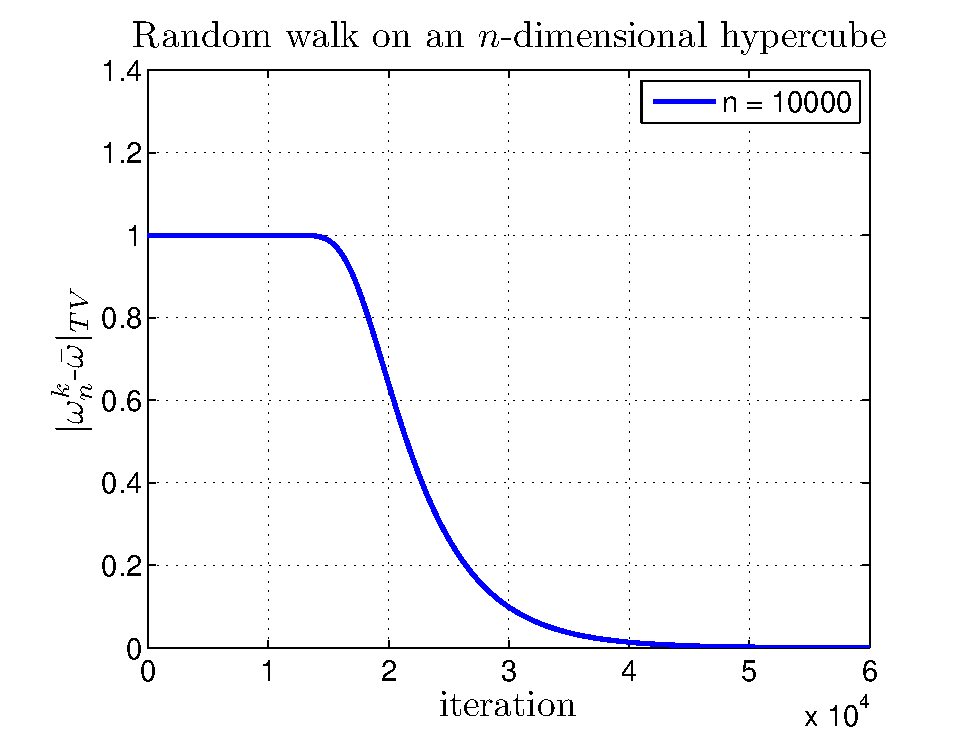
\includegraphics[width=0.45\textwidth,trim=1cm 1cm 0cm 0cm]{rdwalk1}
\parbox[b]{12cm}{
 \begin{itemize}\setlength{\parskip}{0pt}  \setlength{\itemsep}{5pt} \setlength{\topsep}{0pt}
  \item A Markov Chain with $2^n$ states.
  \item The invariant distribution $\bar{\omega}_n$ is uniform. 
  \item $|\omega^k_n - \bar{\omega}_n|_{TV}$, where $k$ is the number of iterations. 
 \end{itemize}
  \textbf{Total Variation Distance}
  \begin{eqnarray*}
   |\mu - \nu|_{TV} = \frac{1}{2}\sum_{i=1}^n |\mu(i)-\nu(i) |
  \\[-2cm]
  \end{eqnarray*}
   }

\end{example} 



%%%%%%%%%%%%%%%%%%%%%%%%%%%%%%%%%%%%%%%%%%%%%%%%%%%%%%%%%%%%%%%%%%%%%%%%%
%%%%%%%%%%%%%%%%%%%%%%%%%%%%%%%%%%%%%%%%%%%%%%%%%%%%%%%%%%%%%%%%%%%%%%%%%
\newpage
\oursection{Cutoff Phenomenon}
%%%%%%%%%%%%%%%%%%%%%%%%%%%%%%%%%%%%%%%%%%%%%%%%%%%%%%%%%%%%%%%%%%%%%%%%%
Assume that, to any
finite set $\Omega$ and any pair of probability measures $\omega$, $\bar{\omega}$ on $\Omega$ is associated a real number
$D(\omega,\bar{\omega})$ such that $D(\omega,\bar{\omega})\in [0,1]$, $\max_{\Omega,\omega,\bar{\omega}} D(\omega,\bar{\omega}) = 1$
and $D(\omega,\bar{\omega})=0$ if and only if $\bar{\omega}=\omega$. Consider a sequence of
(finite) probability spaces $(\Omega_n,\bar{\omega}_n)$, $n=1,2,...$, each equipped with a sequence
of probability measure $\omega^k_n$, $k=0,1,...$, such that
$\lim_{k \rightarrow \infty} D(\omega_n,\bar{\omega}_n)=0$.
The definition of a cutoff is,

\begin{definition}
\label{cutoffdefinition} (Diaconis) A family $(\Omega_n,\bar{\omega}_n, (\omega^k_n)_{k=0,1,...})_{n=1,2,...}$ presents a D-cut-off if
there exists a sequence $(t_n)$ of positive reals such that, for any $\epsilon \in(0,1)$,
\begin{enumerate}
  \item $\lim_{n \rightarrow \infty}D(\omega^{k_n}_n,\bar{\omega}_n) = 0 \mbox{ if }
  k_n>(1+\epsilon)t_n$
  \item $\lim_{n \rightarrow \infty}D(\omega^{k_n}_n,\bar{\omega}_n) = 1 \mbox{ if }
  k_n<(1-\epsilon)t_n $
\end{enumerate}
\end{definition}

%%%%%%%%%%%%%%%%%%%%%%%%%%%%%%%%%%%%%%%%%%%%%%%%%%%%%%%%%%%%%%%%%%%%%%%%%
%%%%%%%%%%%%%%%%%%%%%%%%%%%%%%%%%%%%%%%%%%%%%%%%%%%%%%%%%%%%%%%%%%%%%%%%%
\newpage
\oursection{Cutoff Phenomenon}
%%%%%%%%%%%%%%%%%%%%%%%%%%%%%%%%%%%%%%%%%%%%%%%%%%%%%%%%%%%%%%%%%%%%%%%%%


%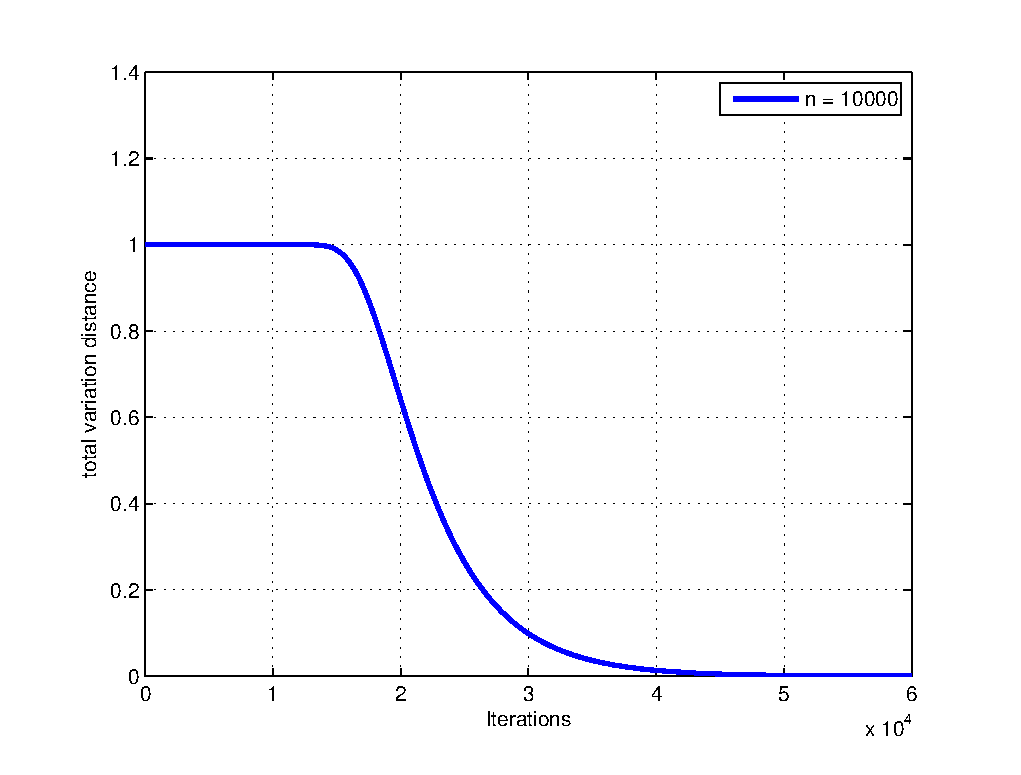
\includegraphics[width=0.45\textwidth,trim=1cm -1cm 0cm 0cm]{cutoffexample}
\centerline{
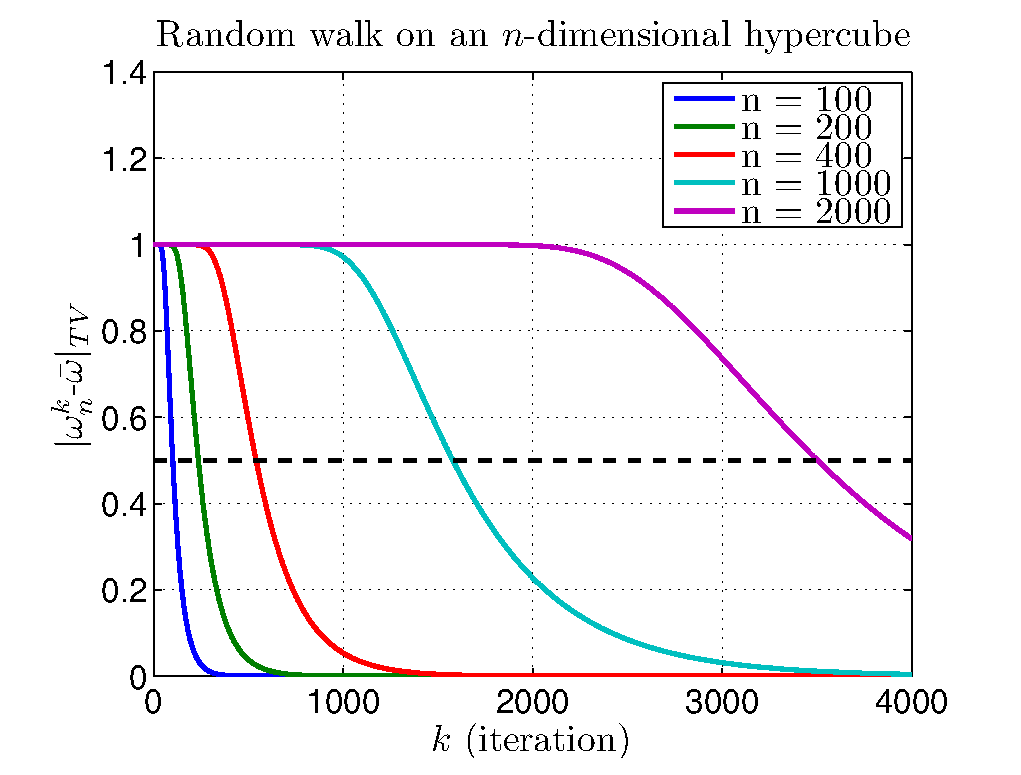
\includegraphics[width=0.43\textwidth,trim=1cm -1cm 0cm 0cm]{rdwalk}
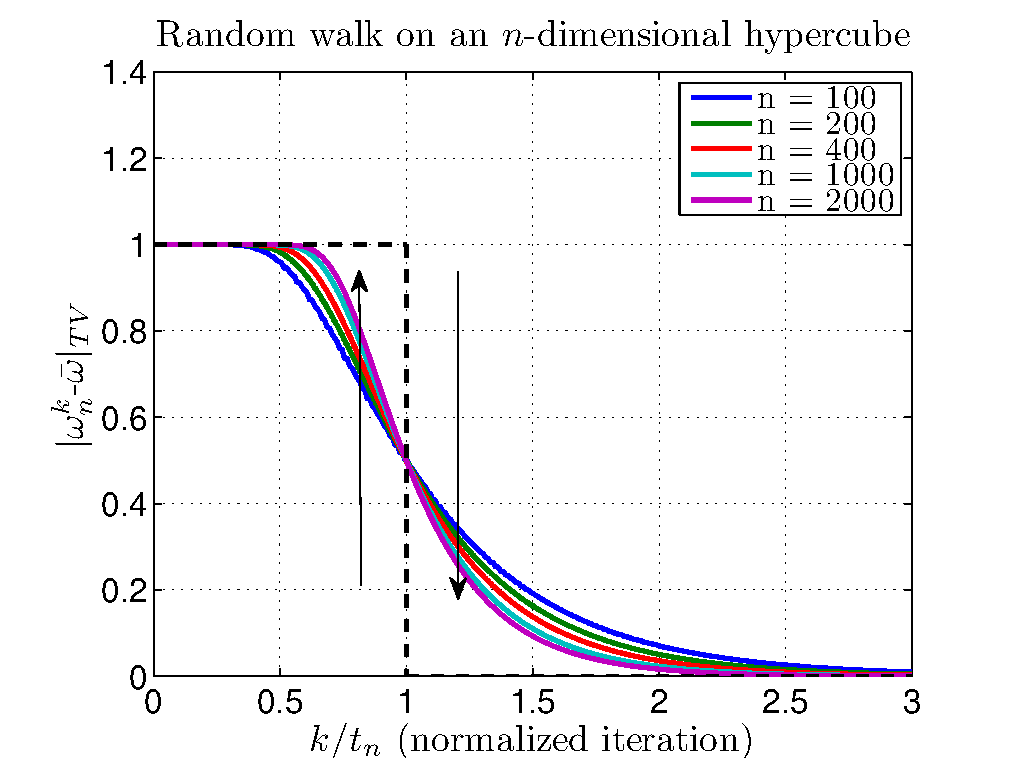
\includegraphics[width=0.43\textwidth,trim=1cm -1cm 0cm 0cm]{rdwalkn}
}
\vspace{-1.5cm}
 \begin{itemize}\setlength{\parskip}{0pt}  \setlength{\itemsep}{5pt} \setlength{\topsep}{0pt}
  \item Distance measure $D$. 
  \item Cutoff time $t_n$.
  \item The behavior of a sequence of Markov chains. 
 \end{itemize}



%%%%%%%%%%%%%%%%%%%%%%%%%%%%%%%%%%%%%%%%%%%%%%%%%%%%%%%%%%%%%%%%%%%%%%%%%
%%%%%%%%%%%%%%%%%%%%%%%%%%%%%%%%%%%%%%%%%%%%%%%%%%%%%%%%%%%%%%%%%%%%%%%%%
\newpage
\oursection{\mytopicb}
%%%%%%%%%%%%%%%%%%%%%%%%%%%%%%%%%%%%%%%%%%%%%%%%%%%%%%%%%%%%%%%%%%%%%%%%%
\begin{itemize}\setlength{\parskip}{0pt}  \setlength{\itemsep}{5pt} \setlength{\topsep}{0pt}
  \item How the variance changes when a scalar function is evolved by a chaotic map and the diffusion goes to zero.
  \item Generating a sequence of Markov chain $A_n$ such that when $n$ goes to infinity, diffusion goes to zero.
  \item Numerical evidence of Standard map cutoffs.
\end{itemize}
Why Standard map?
\vspace{-0.5cm}
\begin{itemize}\setlength{\parskip}{0pt}  \setlength{\itemsep}{5pt} \setlength{\topsep}{0pt}
\item Most researches are focused on the property of the map itself, not the Perron-Frobenius or Koopman operators of it.
\item Known numerical results have poor resolution. ($500 \times 500$).
  We use up to $80000\times 80000$ number of grids. $51.2$ Gbytes of memory is required. %to store a single state vector.
\item The issue of numerical diffusion versus physical diffusion.
\end{itemize}

%%%%%%%%%%%%%%%%%%%%%%%%%%%%%%%%%%%%%%%%%%%%%%%%%%%%%%%%%%%%%%%%%%%%%%%%%
%%%%%%%%%%%%%%%%%%%%%%%%%%%%%%%%%%%%%%%%%%%%%%%%%%%%%%%%%%%%%%%%%%%%%%%%%
\newpage
\oursection{Perron-Frobenius Operator and Koopman Operator}
%%%%%%%%%%%%%%%%%%%%%%%%%%%%%%%%%%%%%%%%%%%%%%%%%%%%%%%%%%%%%%%%%%%%%%%%%
Given a map $S:X \rightarrow X$. In the measure space $(X,\mathcal{A},\mu)$,
\begin{definition} {\bfseries (Perron-Frobenius operator)}
Let $f \in L^1$, for every $A \in \mathcal{A}$ the operator $P:L^1 \rightarrow L^1$ satisfies
  \begin{eqnarray}
    \int_A Pf(x)\mu(dx) = \int_{S^{-1}(A)} f(x)\mu(dx)
  \end{eqnarray}
is the Perron-Frobenius operator associated with $S$.
\end{definition}


\begin{definition} {\bfseries (Koopman operator)}
Let $f \in L^\infty$. The operator $U:L^{\infty} \rightarrow L^{\infty} $ defined by
 \begin{eqnarray}
 Uf(x) = f(S(x))
 \end{eqnarray}
is called the Koopman operator associated with $S$.
\end{definition}
%%%%%%%%%%%%%%%%%%%%%%%%%%%%%%%%%%%%%%%%%%%%%%%%%%%%%%%%%%%%%%%%%%%%%%%%%
%%%%%%%%%%%%%%%%%%%%%%%%%%%%%%%%%%%%%%%%%%%%%%%%%%%%%%%%%%%%%%%%%%%%%%%%%
\newpage
\oursection{Scheme}
%%%%%%%%%%%%%%%%%%%%%%%%%%%%%%%%%%%%%%%%%%%%%%%%%%%%%%%%%%%%%%%%%%%%%%%%%
\begin{itemize}
\item Consider a discrete-time map $S:X\rightarrow X$.
\item Find either the Perron-Frobenius operator or the Koopman operator of $S$. 
\item The operator can be reduced by model reduction techniques. The result is a \textbf{Markov Chain}.
\item Diffusion can be added by a diffusion operator in spatial domain or in frequency domain.  \
%\item This is also the strategy we use to approximate the solution of advection-diffusion equation of mixing channels.
\end{itemize}

%%%%%%%%%%%%%%%%%%%%%%%%%%%%%%%%%%%%%%%%%%%%%%%%%%%%%%%%%%%%%%%%%%%%%%%%%
\newpage
\oursection{Model Reduction}
%%%%%%%%%%%%%%%%%%%%%%%%%%%%%%%%%%%%%%%%%%%%%%%%%%%%%%%%%%%%%%%%%%%%%%%%%

\begin{tabular}{cl}
   \begin{tabular}{c}
      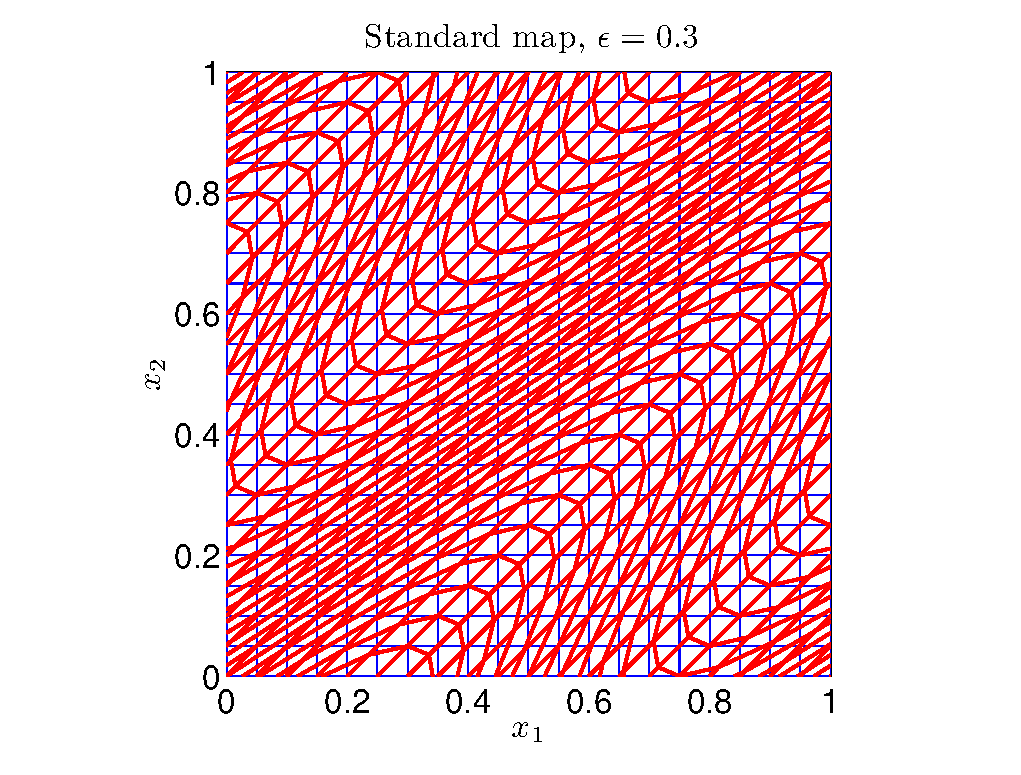
\includegraphics[width=0.45\textwidth,trim=2cm 1cm 2cm 1cm]{standardmapgrid}\\
      \begin{minipage}[s]{9cm}
   \vspace{0.4cm}
%   \begin{equation*}
%   \begin{aligned}
%               x_1' &= x_1+x_2 +\epsilon \sin{2 \pi x_1}  (\mbox{ mod } 1)\\
%               x_2' &=  x_2 +\epsilon \sin{2 \pi x_1}     (\mbox{ mod } 1)
%   \end{aligned}
%   \end{equation*} 
    \begin{eqnarray*}
       \text{Blue grids}:& a_i\\
       \text{Red  grids}:& S^{-1}(a_i)
    \end{eqnarray*}
      \end{minipage}
   \end{tabular}&
  \begin{minipage}[s]{10cm}
   \begin{itemize}
    \item $X = [0,1] \times[0,1]$.
    \item $a_i, i=\{1,2,\cdots,n^2\}$ be regualr $n$ by $n$ grids on $X$.
    \item $\bar{\omega}$ is the invariant measure of $S$.
   \end{itemize}
   The optimal model of Perron-Frobenius operator $A_n$ has 
   \begin{eqnarray}
     \label{Anij}
     (A_n)_{ij} =  \frac{\bar{\omega}(S^{-1}(a_j)\cap a_i)}{\bar{\omega}(a_j)}  \nonumber
    \end{eqnarray} 
   \end{minipage}
\end{tabular}


%   \begin{align}
%               x_1' &= x_1+x_2 \\%+\epsilon \sin{2 \pi x_1}  (\mbox{ mod } 1) \nonumber\\
%               x_2' &=  x_2 %+\epsilon \sin{2 \pi x_1}     (\mbox{ mod } 1)
%   \end{align}

%%%%%%%%%%%%%%%%%%%%%%%%%%%%%%%%%%%%%%%%%%%%%%%%%%%%%%%%%%%%%%%%%%%%%%%%%
%%%%%%%%%%%%%%%%%%%%%%%%%%%%%%%%%%%%%%%%%%%%%%%%%%%%%%%%%%%%%%%%%%%%%%%%%
\newpage
\oursection{Standard Map}
%%%%%%%%%%%%%%%%%%%%%%%%%%%%%%%%%%%%%%%%%%%%%%%%%%%%%%%%%%%%%%%%%%%%%%%%%
\vspace{-0.1cm}
\centerline{
\begin{tabular}{rl}%\setlength{\tabcolsep}{-30mm}
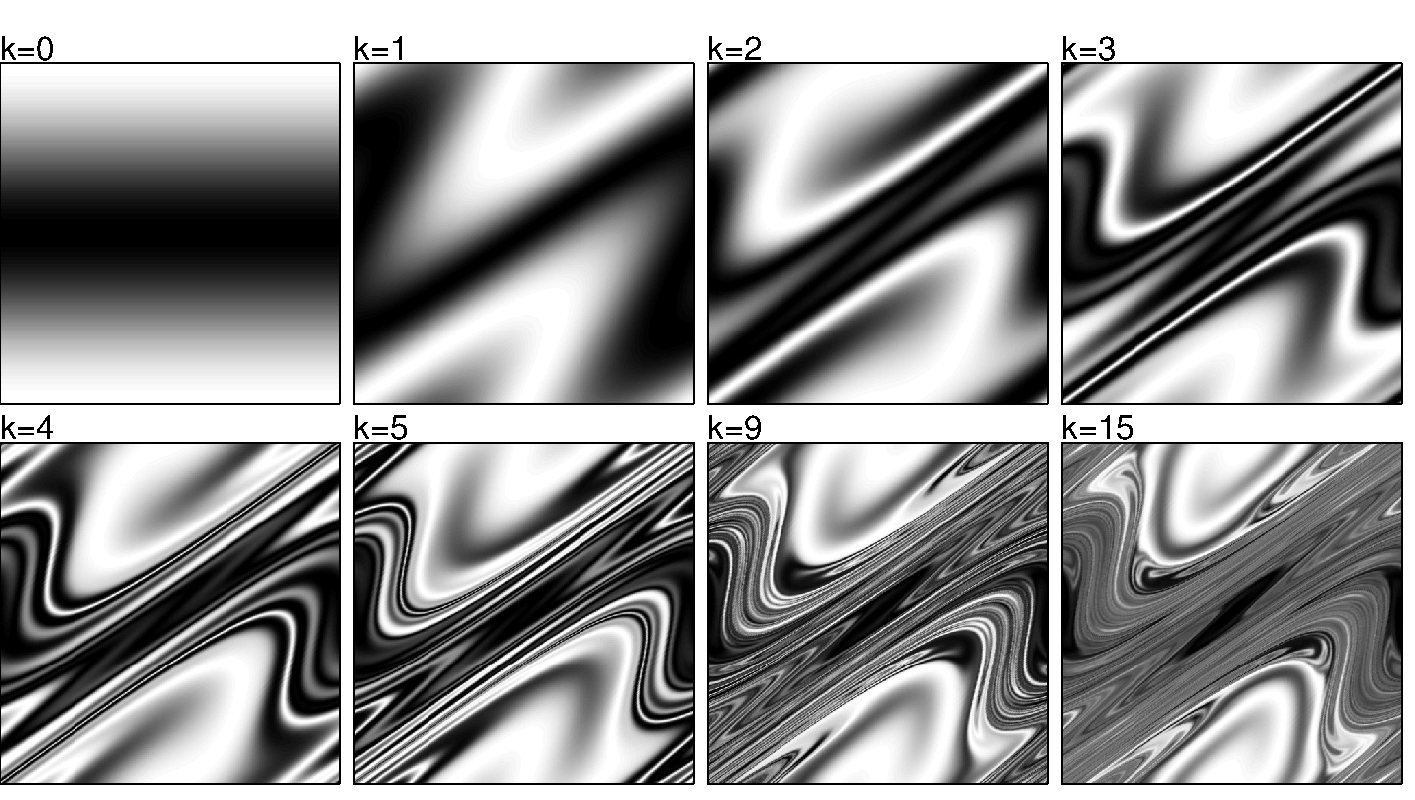
\includegraphics[width=0.75\textwidth,trim=1cm 1cm 0cm 0cm]{standardmapevolve}
%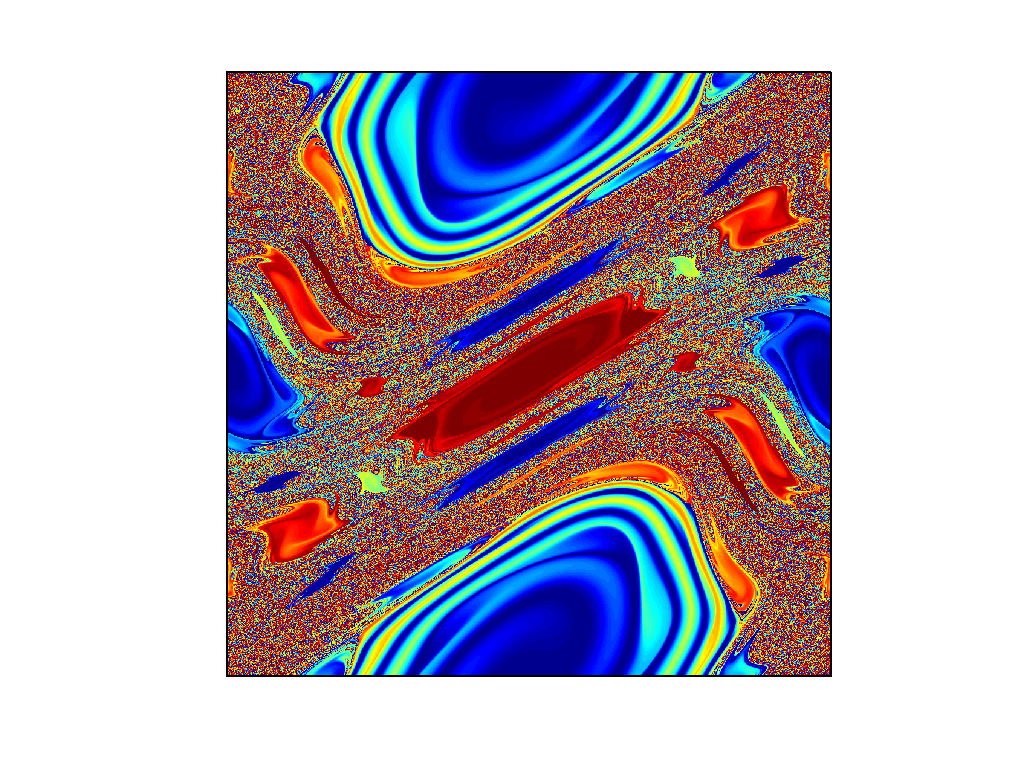
\includegraphics[width=0.52\textwidth,trim=1cm 1cm 0cm 0cm]{standardmapsimuexact}&
%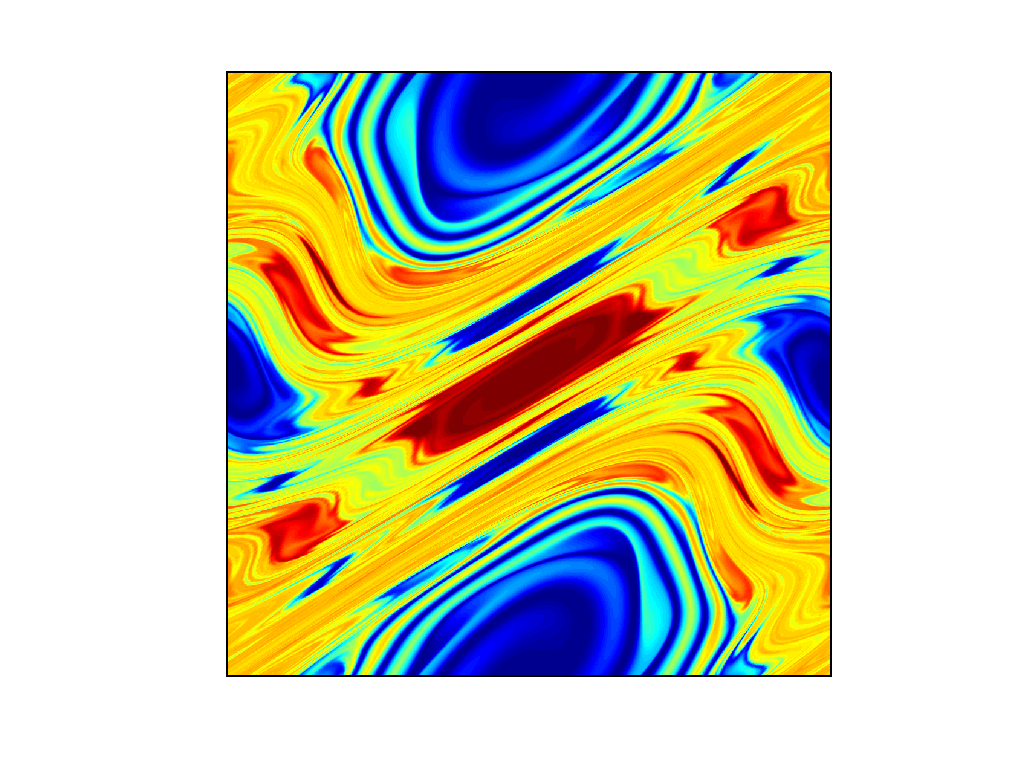
\includegraphics[width=0.52\textwidth,trim=1cm 1cm 0cm 0cm]{standardmapsimumarkov}
\end{tabular}
}
   \begin{equation*}
     \begin{cases}
        x_1' = &x_1+x_2 +\epsilon \sin{2 \pi x_1}  (\mbox{ mod } 1)\\
        x_2' = & x_2 +\epsilon \sin{2 \pi x_1}     (\mbox{ mod } 1) 
     \end{cases}     
   \end{equation*}
   \begin{equation*}
      \epsilon=0.3, \,\, f^0   = \cos(2\pi x_2)
   \end{equation*}





%%%%%%%%%%%%%%%%%%%%%%%%%%%%%%%%%%%%%%%%%%%%%%%%%%%%%%%%%%%%%%%%%%%%%%%%%
%%%%%%%%%%%%%%%%%%%%%%%%%%%%%%%%%%%%%%%%%%%%%%%%%%%%%%%%%%%%%%%%%%%%%%%%%
%\newpage
%\oursection{Standard Map Simulation in Frequency Domain}
%%%%%%%%%%%%%%%%%%%%%%%%%%%%%%%%%%%%%%%%%%%%%%%%%%%%%%%%%%%%%%%%%%%%%%%%%
%\centerline{
%\begin{tabular}{rl}%\setlength{\tabcolsep}{-30mm}
%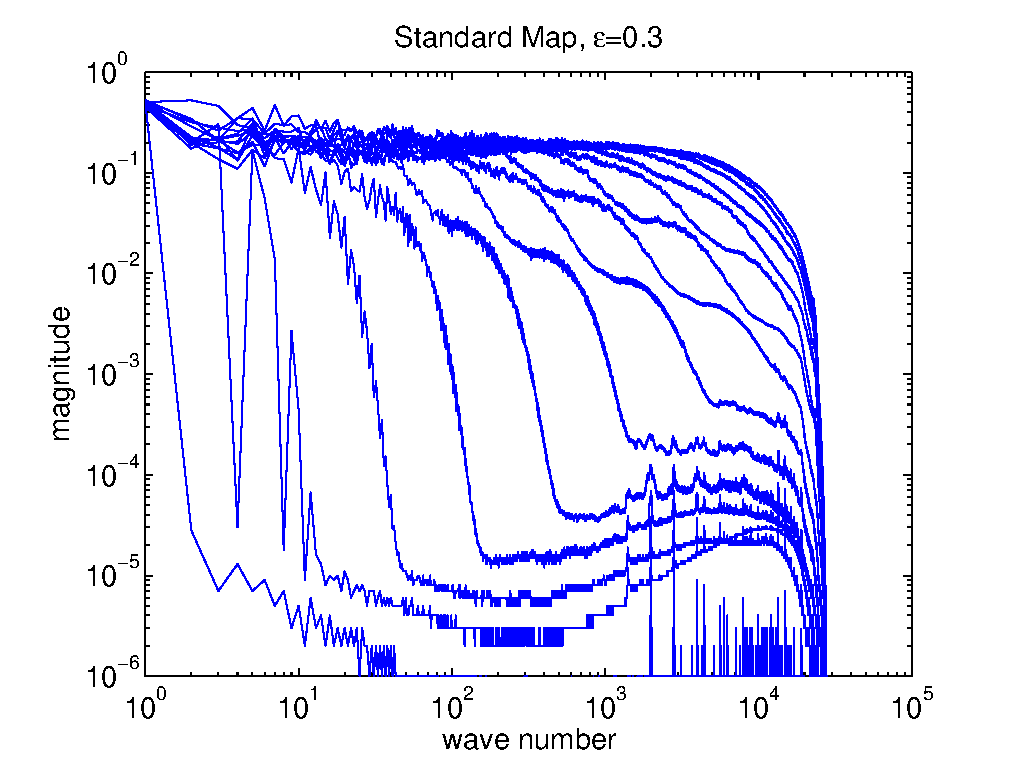
\includegraphics[width=0.55\textwidth,trim=1cm 1cm 0cm 0cm]{standardmapfreqevolve}&
%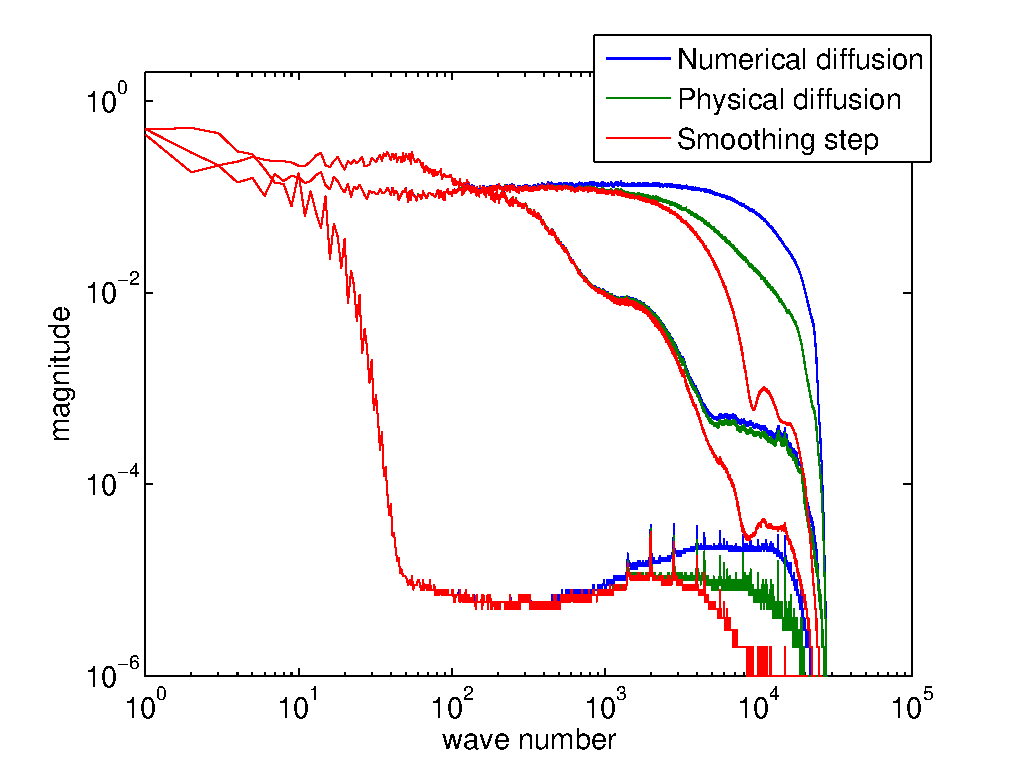
\includegraphics[width=0.55\textwidth,trim=1cm 1cm 0cm 0cm]{standardmapfreqcompare}
%\end{tabular}
%}


%%%%%%%%%%%%%%%%%%%%%%%%%%%%%%%%%%%%%%%%%%%%%%%%%%%%%%%%%%%%%%%%%%%%%%%%%
%%%%%%%%%%%%%%%%%%%%%%%%%%%%%%%%%%%%%%%%%%%%%%%%%%%%%%%%%%%%%%%%%%%%%%%%%
\newpage
\oursection{Evidence of Standard Map Cutoff}
%%%%%%%%%%%%%%%%%%%%%%%%%%%%%%%%%%%%%%%%%%%%%%%%%%%%%%%%%%%%%%%%%%%%%%%%%
\centerline{
\begin{tabular}{rl}%\setlength{\tabcolsep}{-30mm}
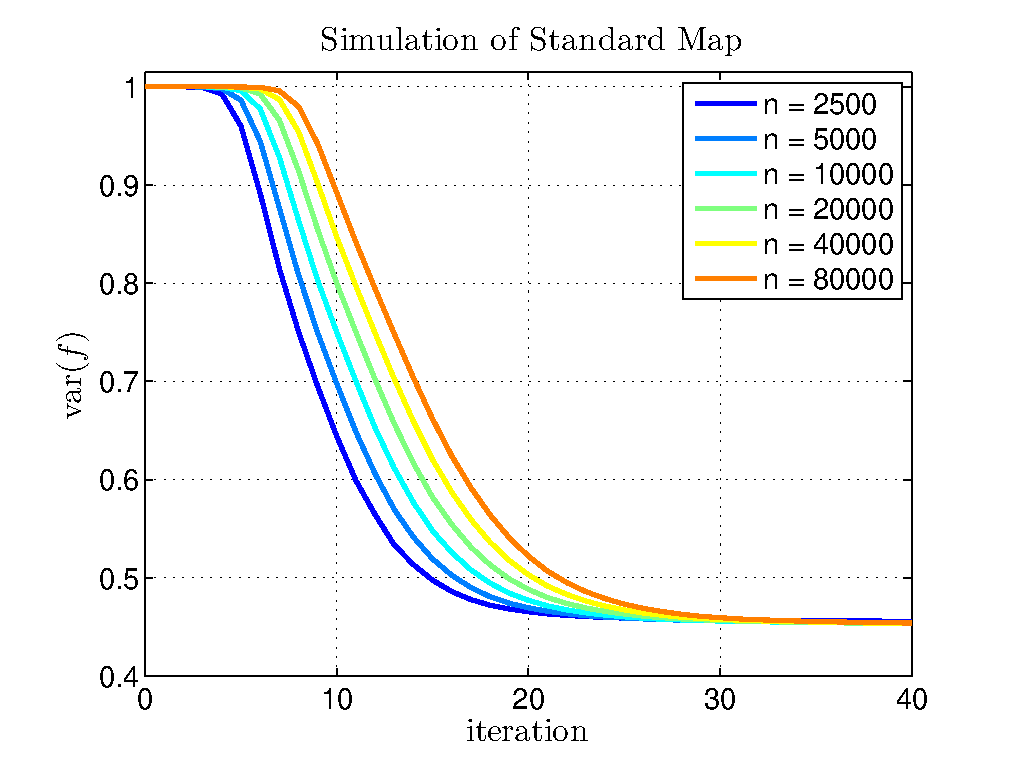
\includegraphics[width=0.55\textwidth,trim=1cm 1cm 0cm 0cm]{standardmapcutoff}&
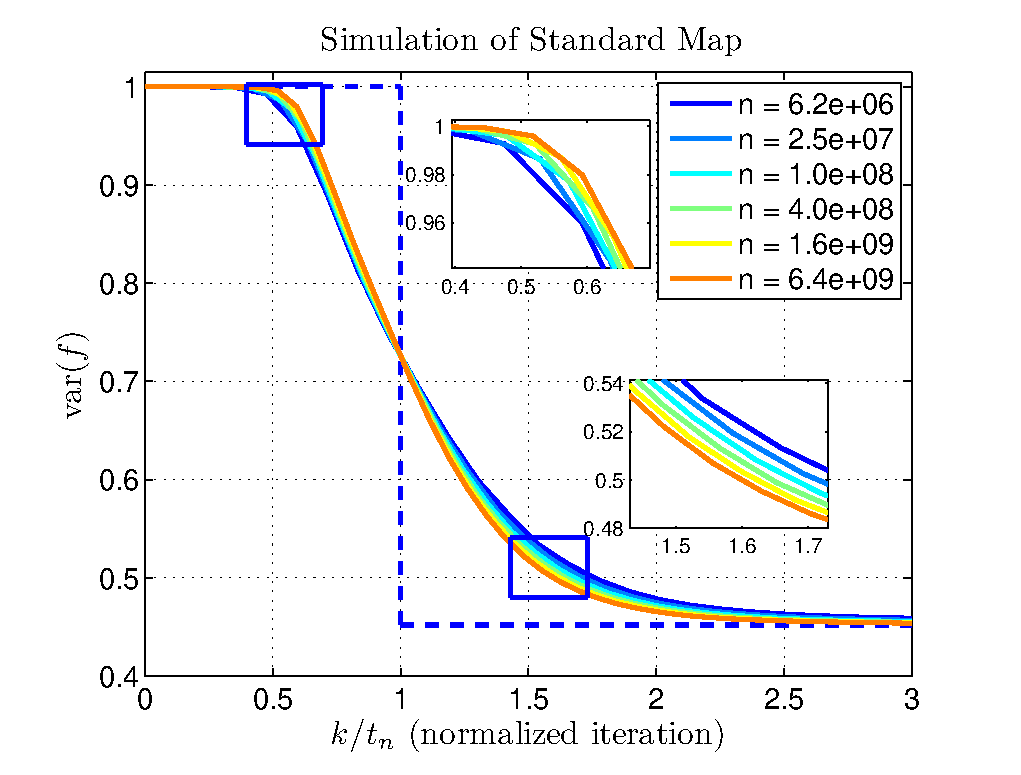
\includegraphics[width=0.55\textwidth,trim=1cm 1cm 0cm 0cm]{standardmapcutoffn}
\end{tabular}
}
\begin{itemize}\setlength{\parskip}{0pt}  \setlength{\itemsep}{5pt} \setlength{\topsep}{0pt}
\item Standard map, $\epsilon = 0.3$, $f^0 = \cos(2\pi x_2)$.
\item $(M,m) = (1,0.4521)$, Cutoff time: $t_n =\min \{ k \mid \text{var}(f^k_n)< \frac{M+m}{2}\} $
\end{itemize}
%%%%%%%%%%%%%%%%%%%%%%%%%%%%%%%%%%%%%%%%%%%%%%%%%%%%%%%%%%%%%%%%%%%%%%%%%
%%%%%%%%%%%%%%%%%%%%%%%%%%%%%%%%%%%%%%%%%%%%%%%%%%%%%%%%%%%%%%%%%%%%%%%%%
%\newpage
%\oursection{Evidence of Standard Map Cutoff}
%%%%%%%%%%%%%%%%%%%%%%%%%%%%%%%%%%%%%%%%%%%%%%%%%%%%%%%%%%%%%%%%%%%%%%%%%
%\centerline{
%\begin{tabular}{rl}%\setlength{\tabcolsep}{-30mm}
%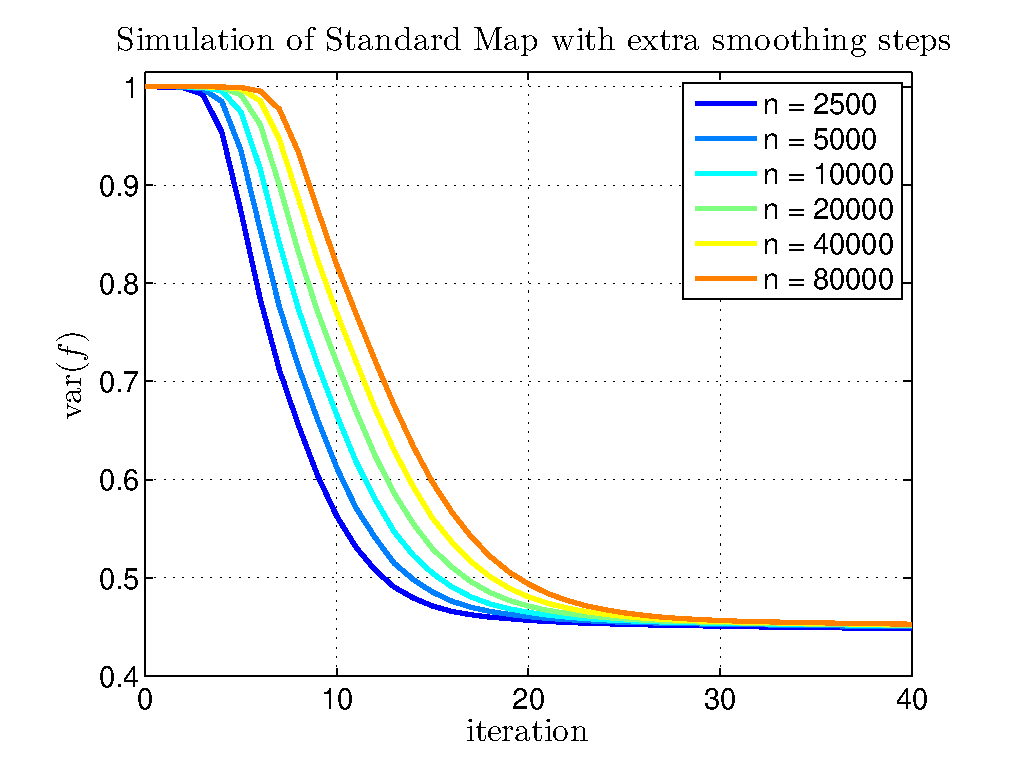
\includegraphics[width=0.55\textwidth,trim=1cm 1cm 0cm 0cm]{standardmapcutoffwithsmoothing}&
%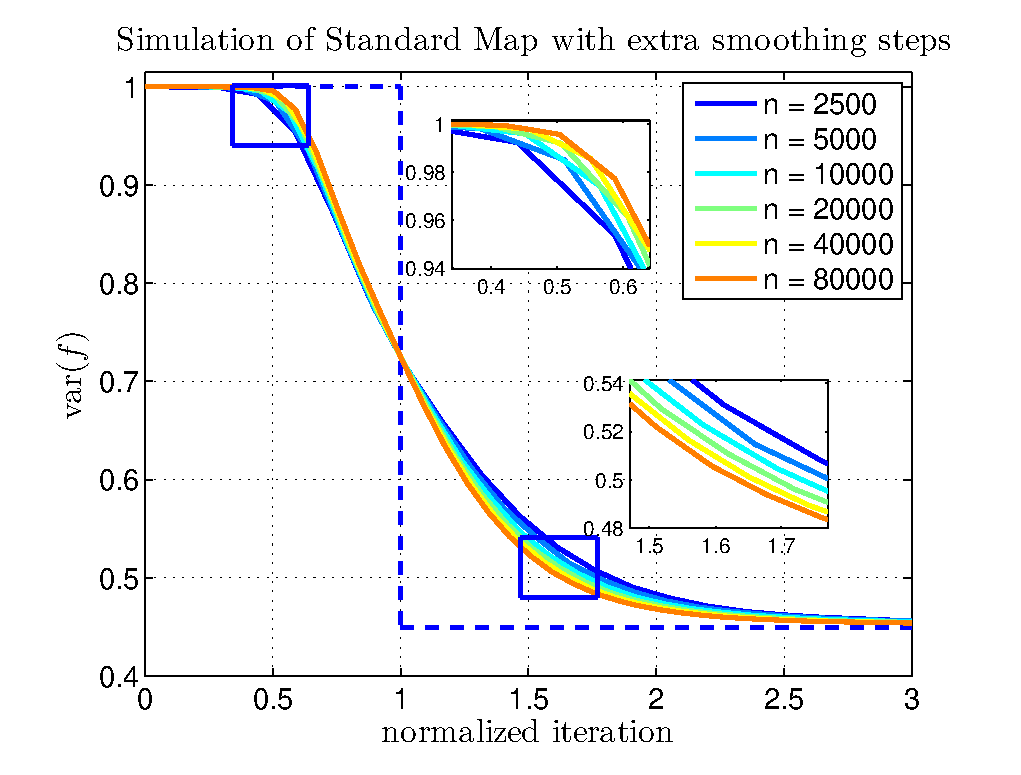
\includegraphics[width=0.55\textwidth,trim=1cm 1cm 0cm 0cm]{standardmapcutoffwithsmoothingn}
%\end{tabular}
%}

%\begin{itemize}\setlength{\parskip}{0pt}  \setlength{\itemsep}{5pt} \setlength{\topsep}{0pt}
%\item Standard map, $\epsilon = 0.3$, $f^0 = \cos(2\pi x_2)$, with additional smoothing steps after each iteration.
%\item $(M,m) = (1,0.4498)$, Cutoff time: $t_n =\min \{ k \mid \text{var}(f^k_n)< \frac{M+m}{2}\} $
%\end{itemize}

%%%%%%%%%%%%%%%%%%%%%%%%%%%%%%%%%%%%%%%%%%%%%%%%%%%%%%%%%%%%%%%%%%%%%%%%%
%%%%%%%%%%%%%%%%%%%%%%%%%%%%%%%%%%%%%%%%%%%%%%%%%%%%%%%%%%%%%%%%%%%%%%%%%
\newpage
\oursection{Evidence of Standard Map Cutoff}
%%%%%%%%%%%%%%%%%%%%%%%%%%%%%%%%%%%%%%%%%%%%%%%%%%%%%%%%%%%%%%%%%%%%%%%%%
\centerline{
\begin{tabular}{rl}%\setlength{\tabcolsep}{-30mm}
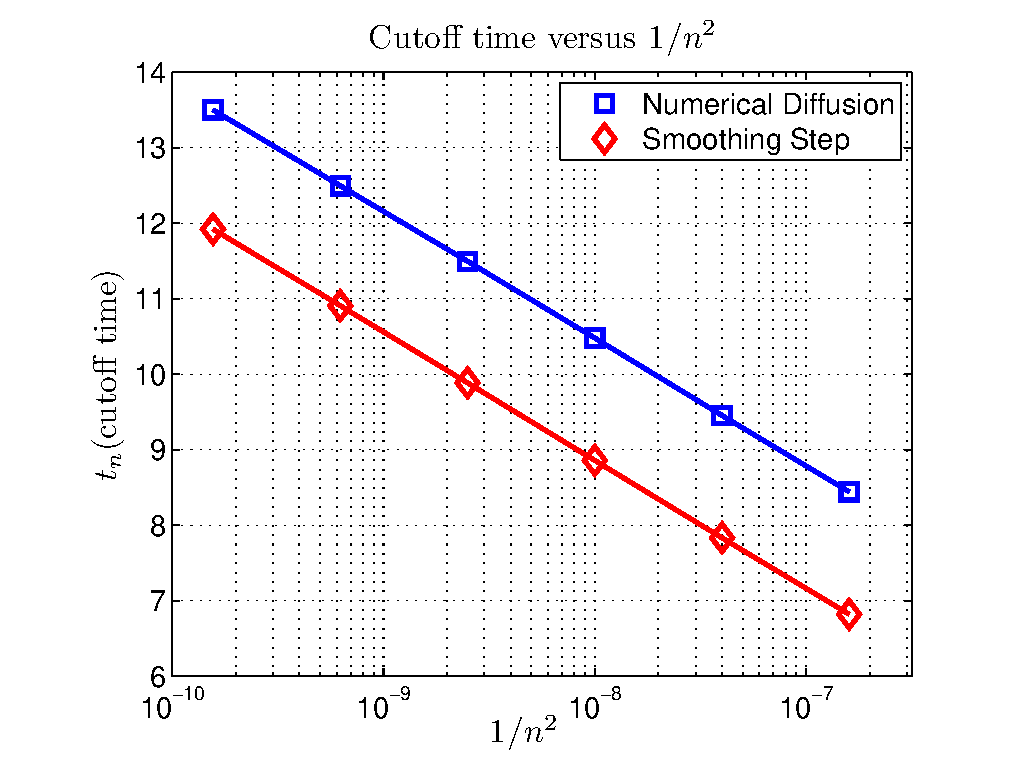
\includegraphics[width=0.55\textwidth,trim=1cm 1cm 0cm 0cm]{cutofftimevsD}&
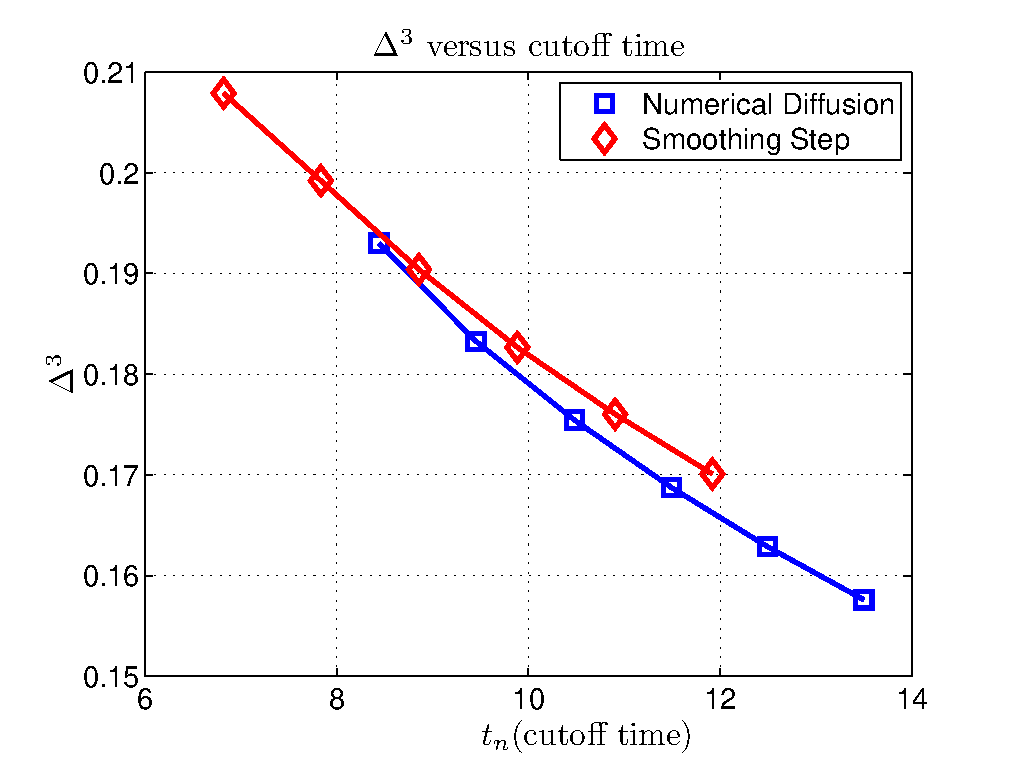
\includegraphics[width=0.55\textwidth,trim=1cm 1cm 0cm 0cm]{areavscutofftime}
\end{tabular}
}
\begin{itemize}\setlength{\parskip}{0pt}  \setlength{\itemsep}{5pt} \setlength{\topsep}{0pt}
\item Cutoff time: $t_n =\min \{ k \mid \text{var}(f^k_n)< \frac{M+m}{2}\} $.
\item $\Delta^l\equiv \int_0^l | \nu_{\infty}(x)-\nu_{n}(x)|dx$.
\end{itemize}
%%%%%%%%%%%%%%%%%%%%%%%%%%%%%%%%%%%%%%%%%%%%%%%%%%%%%%%%%%%%%%%%%%%%%%%%%
\newpage
\oursection{Conclusion}
%%%%%%%%%%%%%%%%%%%%%%%%%%%%%%%%%%%%%%%%%%%%%%%%%%%%%%%%%%%%%%%%%%%%%%%%%
%%%%%%%%%%%%%%%%%%%%%%%%%%%%%%%%%%%%%%%%%%%%%%%%%%%%%%%%%%%%%%%%%%%%%%%%%
\begin{itemize}
  \item We bring the definition of cutoff phenomenon to characterize the chaotic mixing.
  \item Numerical evidence of Standard map cutoff.
  \item It is really a cutoff!
\end{itemize}


%%%%%%%%%%%%%%%%%%%%%%%%%%%%%%%%%%%%%%%%%%%%%%%%%%%%%%%%%%%%%%%%%%%%%%%%%
%%%%%%%%%%%%%%%%%%%%%%%%%%%%%%%%%%%%%%%%%%%%%%%%%%%%%%%%%%%%%%%%%%%%%%%%%
%%%%%%%%%%%%%                 TOPIC b                          %%%%%%%%%%
%%%%%%%%%%%%%%%%%%%%%%%%%%%%%%%%%%%%%%%%%%%%%%%%%%%%%%%%%%%%%%%%%%%%%%%%%
%%%%%%%%%%%%%%%%%%%%%%%%%%%%%%%%%%%%%%%%%%%%%%%%%%%%%%%%%%%%%%%%%%%%%%%%%

\newpage
\oursection{\mytopicc}
   \begin{itemize}
      \item Tent map ``cutoff''
      \item Random Walks on an $n$-dimensional hypercubes
      \item Symbolic Dynamics and Stochastic Symbol sequence
      \item Create Cutoffs 
   \end{itemize}
%%%%%%%%%%%%%%%%%%%%%%%%%%%%%%%%%%%%%%%%%%%%%%%%%%%%%%%%%%%%%%%%%%%%%%%%%
%%%%%%%%%%%%%%%%%%%%%%%%%%%%%%%%%%%%%%%%%%%%%%%%%%%%%%%%%%%%%%%%%%%%%%%%%
\newpage
\oursection{Tent Map ``Cutoff''}
%%%%%%%%%%%%%%%%%%%%%%%%%%%%%%%%%%%%%%%%%%%%%%%%%%%%%%%%%%%%%%%%%%%%%%%%%
%\begin{example} %\textbf{Tent Map}
%\begin{figure}
\centerline{
\begin{tabular}{rcl}
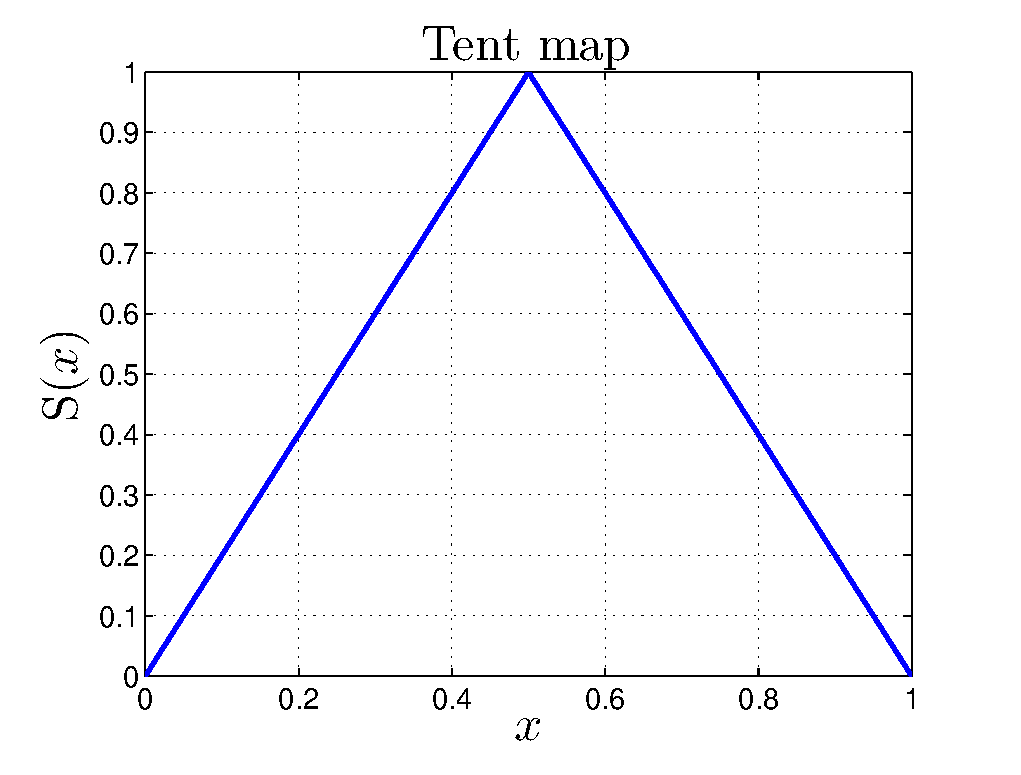
\includegraphics[width=0.34\textwidth,trim=1cm 1cm 1cm 1cm]{tentmap}&
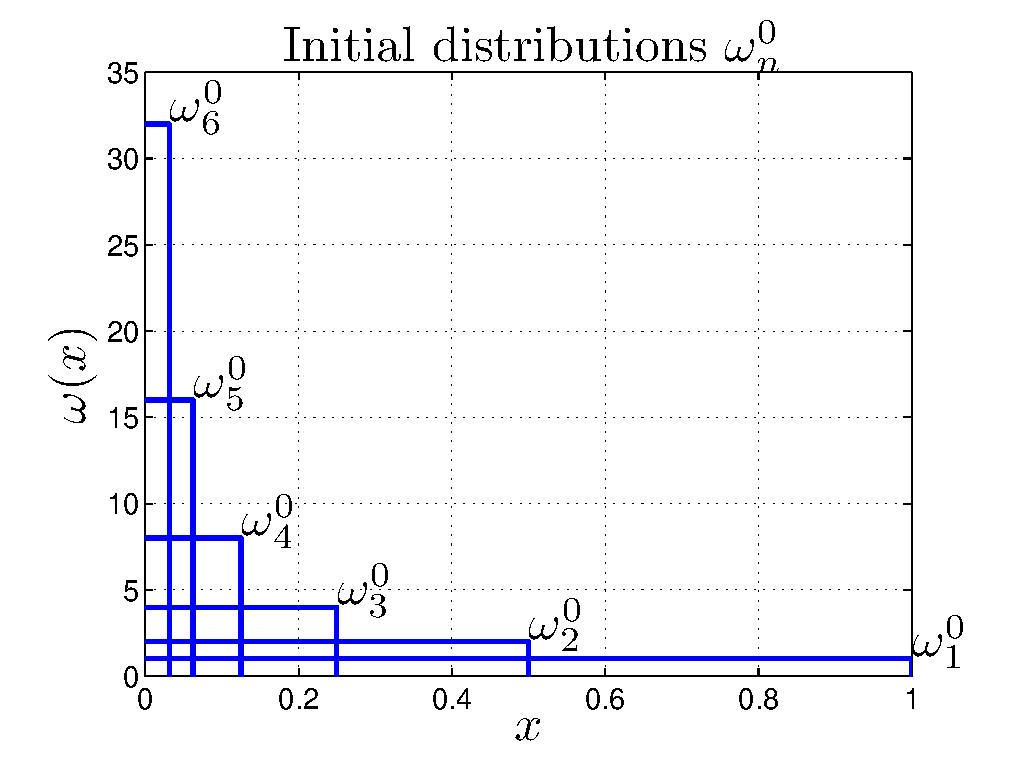
\includegraphics[width=0.34\textwidth,trim=1cm 1cm 1cm 1cm]{tentmapomega0}&
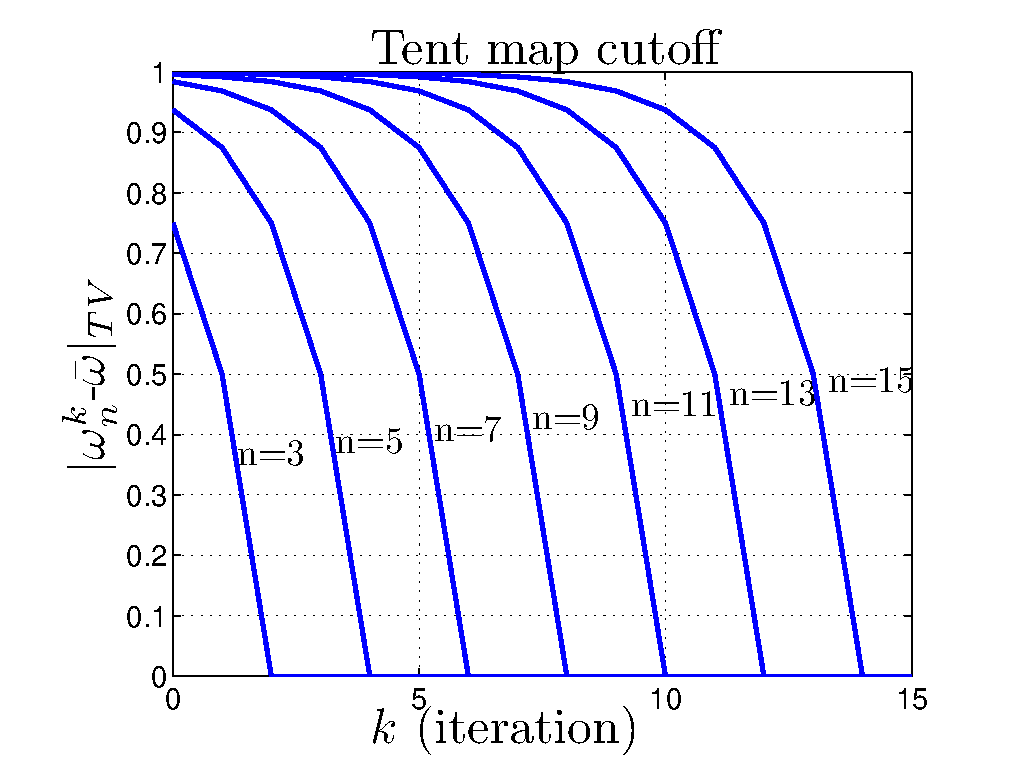
\includegraphics[width=0.34\textwidth,trim=1cm 1cm 1cm 1cm]{tentmapcutoff}
\end{tabular}
}
%\end{figure}
\vspace{-1cm}
   \begin{eqnarray}
   \label{tentmapevolve}
     x' = S_\text{tent}(x) \equiv 1-2\left|x-\frac{1}{2}\right|,\,\,\,
     \omega_n^{k+1}(x) = \frac{1}{2}\left(\omega_n^k\left(\frac{x}{2}\right)+\omega_n^k\left(1-\frac{x}{2}\right) \right)
   \\[-1.4cm] \nonumber
   \end{eqnarray}
with the following initial distributions on $[0 ,1]$,
  \begin{eqnarray}
  \label{tentmapinitial}
  \\[-1.8cm] \nonumber
    \omega_n^0 = \left\{ \begin{tabular}{c}
                      $\frac{1}{\mu_n}$, \mbox{  if  } $x \le \mu_n$\\
                      $0$, \mbox{  otherwise}
                      \end{tabular}\right.
  \\[-1.6cm] \nonumber
  \end{eqnarray}
where $\mu_1 = 1$, and $\mu_{n+1} = \frac{\mu_n}{2}$.

%\end{example}

%%%%%%%%%%%%%%%%%%%%%%%%%%%%%%%%%%%%%%%%%%%%%%%%%%%%%%%%%%%%%%%%%%%%%%%%%
%%%%%%%%%%%%%%%%%%%%%%%%%%%%%%%%%%%%%%%%%%%%%%%%%%%%%%%%%%%%%%%%%%%%%%%%%
\newpage
\oursection{Revisit random walk on an $n$-dimensional hypercube}
%%%%%%%%%%%%%%%%%%%%%%%%%%%%%%%%%%%%%%%%%%%%%%%%%%%%%%%%%%%%%%%%%%%%%%%%%
\begin{example} \textbf{Random walk on an $n$-dimensional hypercube}
a particle starts at $\mathbf{0}$ and moves to one of its nearest neighbors (or stay fixed) with equal probability at each step.

%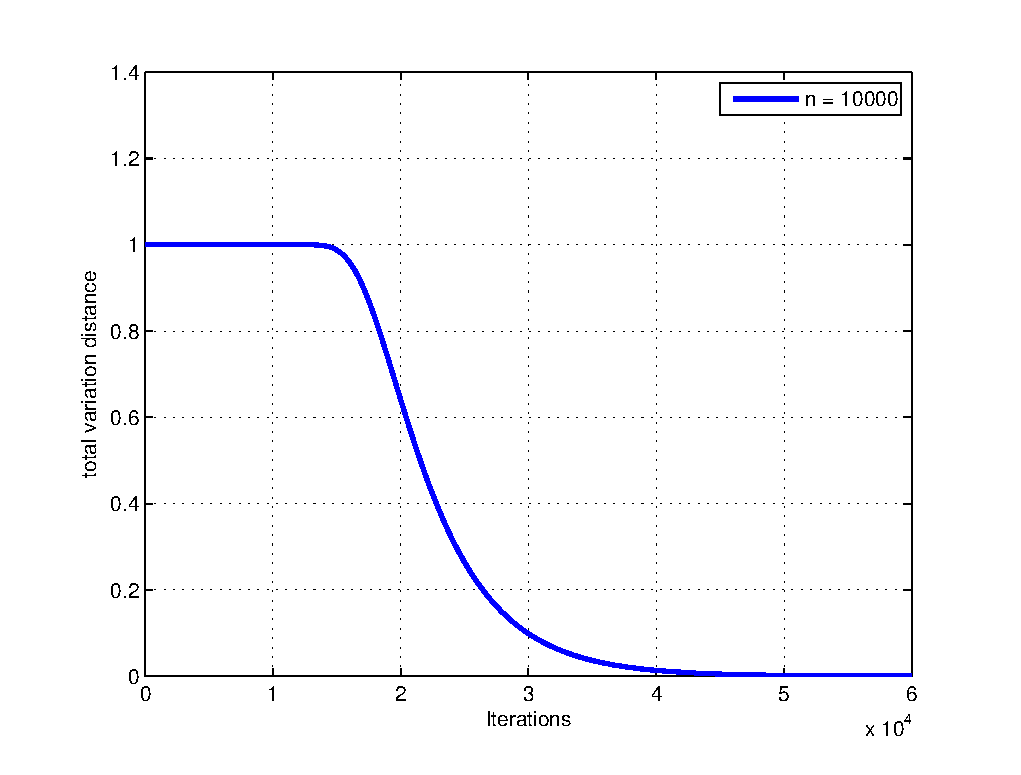
\includegraphics[width=0.45\textwidth,trim=1cm -1cm 0cm 0cm]{cutoffexample}
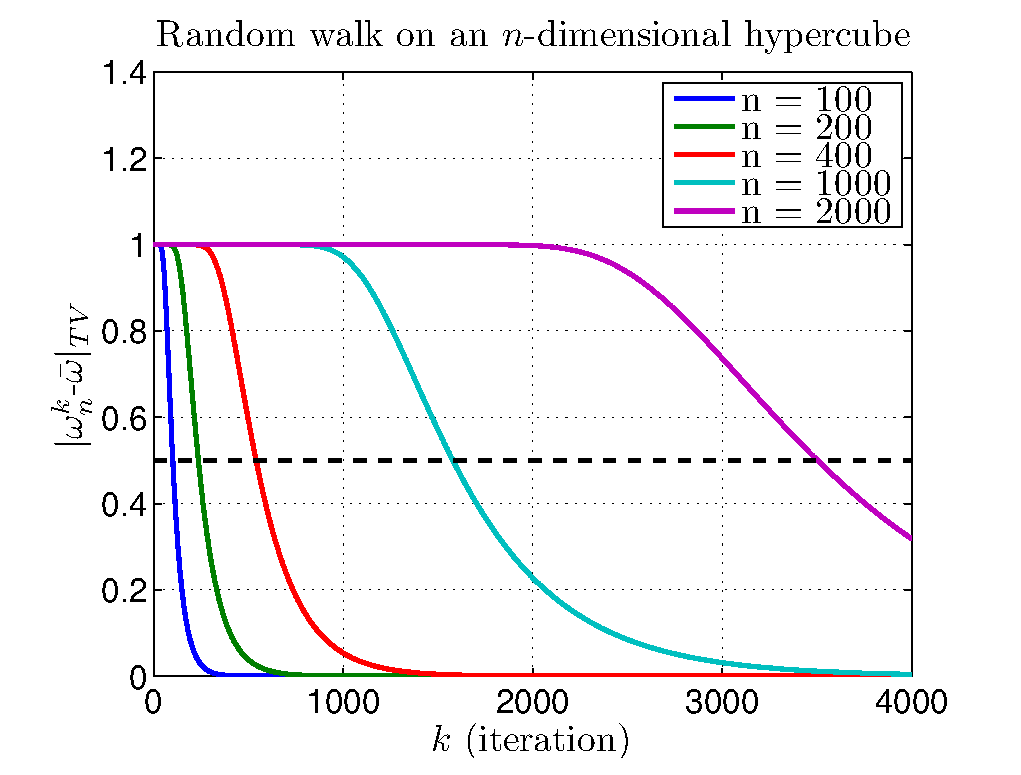
\includegraphics[width=0.45\textwidth,trim=1cm -1cm 0cm 0cm]{rdwalk}
\parbox[b]{12cm}{
  (Diaconis 1990)Let $k = \frac{1}{4}n\log{n}+cn$. Then for fixed $c \in \{-\infty,\infty\}$, as $n \rightarrow \infty$,
\begin{eqnarray}
\label{rdwalkshape}
 |\omega^k_n - \bar{\omega} |_{TV} \sim \erf\left(\frac{e^{-2c}}{\sqrt{8}}\right)
\end{eqnarray}
   }

\end{example}



%%%%%%%%%%%%%%%%%%%%%%%%%%%%%%%%%%%%%%%%%%%%%%%%%%%%%%%%%%%%%%%%%%%%%%%%%
%%%%%%%%%%%%%%%%%%%%%%%%%%%%%%%%%%%%%%%%%%%%%%%%%%%%%%%%%%%%%%%%%%%%%%%%%
\newpage
\oursection{Our Goal}
%%%%%%%%%%%%%%%%%%%%%%%%%%%%%%%%%%%%%%%%%%%%%%%%%%%%%%%%%%%%%%%%%%%%%%%%%
\begin{itemize}
\item Goal: Generate a sequence of $\omega_n^0$ such that when they are evolved by a chaotic map, $|\omega_n^k-\bar{\omega}|_{TV}$ has the same limiting behavior as one sees in the random walk on an $n$-dimensional hypercube problem.
\end{itemize}
We do:
\begin{itemize}
\item Observe why RW has the ``normal'' cutoff shape.
\item Overcome the problem of evolving $\omega_n^k$ for a set of $\omega_n^0\in\bar{\Omega}$, by extending the symbolic dynamics of chaotic maps.
\item Find the upper and lower bounds of $|\omega_n^k-\bar{\omega}|_{TV}$, which characterize the limiting behavior of it.
\end{itemize}


%%%%%%%%%%%%%%%%%%%%%%%%%%%%%%%%%%%%%%%%%%%%%%%%%%%%%%%%%%%%%%%%%%%%%%%%%
%%%%%%%%%%%%%%%%%%%%%%%%%%%%%%%%%%%%%%%%%%%%%%%%%%%%%%%%%%%%%%%%%%%%%%%%%
\newpage
\oursection{What creates the ``normal'' shape?\\ A Model Reduction View}
%%%%%%%%%%%%%%%%%%%%%%%%%%%%%%%%%%%%%%%%%%%%%%%%%%%%%%%%%%%%%%%%%%%%%%%%%

Ehrenfests' Urn Problem
\begin{itemize}%\setlength{\parskip}{0pt}  \setlength{\itemsep}{5pt} \setlength{\topsep}{0pt}
\item Two urns and $n$ balls. To start, all the balls are in urn $1$. Each time, a ball is randomly chosen and moved to the other urn.
\item The state of the Markov chain is the number of balls in urn $1$.
\item The system has $n+1$ states, and $\bar{\omega}(i) = {n \choose i}/2^n$.
\item This problem is equivalent to the random walk on a hypercube problem--as if we put all the states having equal distance to $\mathbf{0}$ together to becomes a new state.
\end{itemize}


%%%%%%%%%%%%%%%%%%%%%%%%%%%%%%%%%%%%%%%%%%%%%%%%%%%%%%%%%%%%%%%%%%%%%%%%%
%%%%%%%%%%%%%%%%%%%%%%%%%%%%%%%%%%%%%%%%%%%%%%%%%%%%%%%%%%%%%%%%%%%%%%%%%
\newpage
\oursection{What creates the ``normal'' shape?\\ A Model Reduction View}
%%%%%%%%%%%%%%%%%%%%%%%%%%%%%%%%%%%%%%%%%%%%%%%%%%%%%%%%%%%%%%%%%%%%%%%%%


\centerline{
\scalebox{0.6}[0.6]{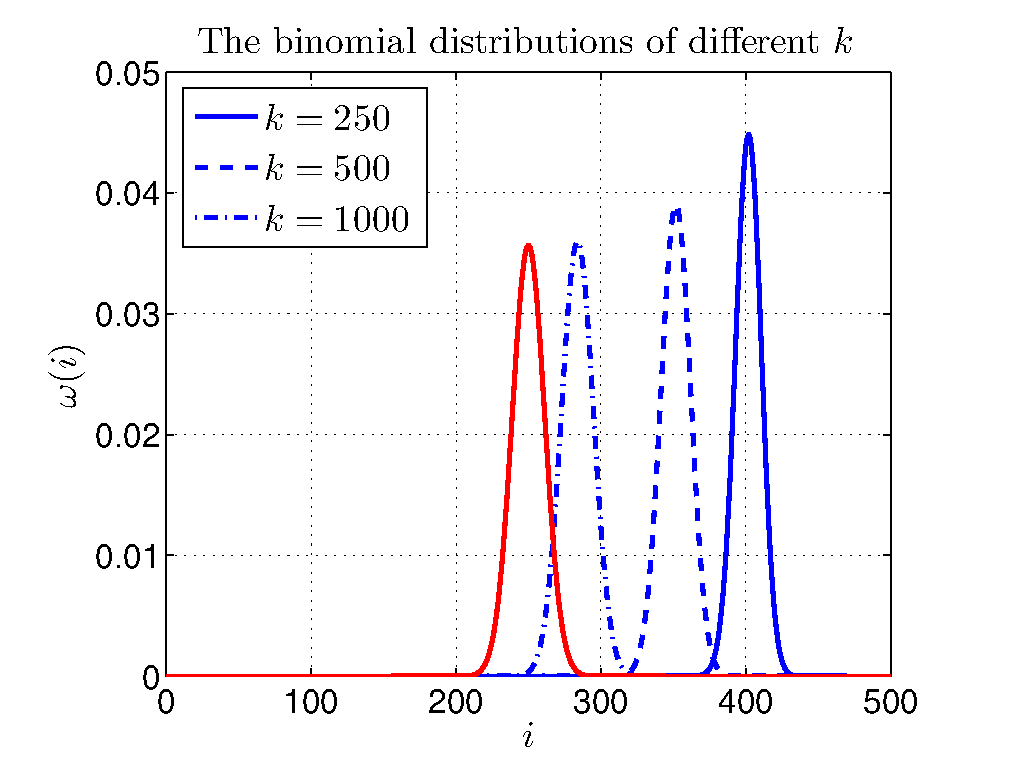
\includegraphics{deltaMexample2a}}
            \scalebox{0.6}[0.6]{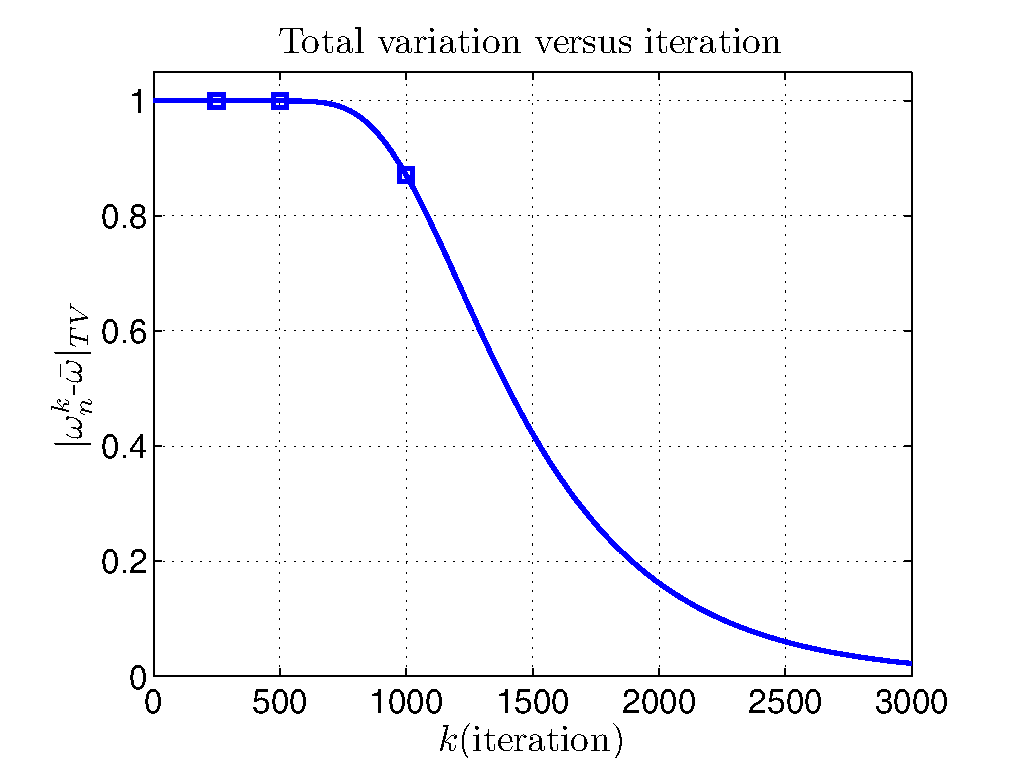
\includegraphics{ehrenfasttv}}
}
\begin{itemize}
\item When $n$ is large, binomial distribution converges normal distribution.
\item The TV between two normal distributions converges to an error function.
\end{itemize}
%%%%%%%%%%%%%%%%%%%%%%%%%%%%%%%%%%%%%%%%%%%%%%%%%%%%%%%%%%%%%%%%%%%%%%%%%
%%%%%%%%%%%%%%%%%%%%%%%%%%%%%%%%%%%%%%%%%%%%%%%%%%%%%%%%%%%%%%%%%%%%%%%%%
\newpage
\oursection{Symbolic Dynamics(for $1$-D Chaotic Maps) }
%%%%%%%%%%%%%%%%%%%%%%%%%%%%%%%%%%%%%%%%%%%%%%%%%%%%%%%%%%%%%%%%%%%%%%%%%

\begin{itemize}\setlength{\parskip}{0pt}  \setlength{\itemsep}{5pt} \setlength{\topsep}{0pt}
     \item Symbol list $\mathcal{S} = \{L,R\}$. Map $S$ has invariant set $\Lambda$, $x\in \Lambda$
     \item  $s_i \in \mathcal{S}$, $s= \{.s_0s_1\cdots s_n\cdots\} \in \Sigma$
     \item  $\phi: \Lambda \rightarrow \Sigma$
     \item $\sigma: \Sigma \rightarrow \Sigma $, shift operator
           $$\sigma(s)= \{.s_1s_2\cdots s_n\cdots\}$$
     \item $S(x) = \phi^{-1}\circ \sigma \circ \phi(x)$,
           \begin{equation*}
          \xymatrix{
              \Lambda  \ar[d]_{\phi} \ar[r]^{S}
              & \Lambda   \ar[d]^{\phi} \\
          \Sigma \ar[r]_{\sigma}
              & \Sigma}
           \end{equation*}
\end{itemize}

%%%%%%%%%%%%%%%%%%%%%%%%%%%%%%%%%%%%%%%%%%%%%%%%%%%%%%%%%%%%%%%%%%%%%%%%%
%%%%%%%%%%%%%%%%%%%%%%%%%%%%%%%%%%%%%%%%%%%%%%%%%%%%%%%%%%%%%%%%%%%%%%%%%
\newpage
\oursection{Symbolic Dynamics }
%%%%%%%%%%%%%%%%%%%%%%%%%%%%%%%%%%%%%%%%%%%%%%%%%%%%%%%%%%%%%%%%%%%%%%%%%

\centerline{
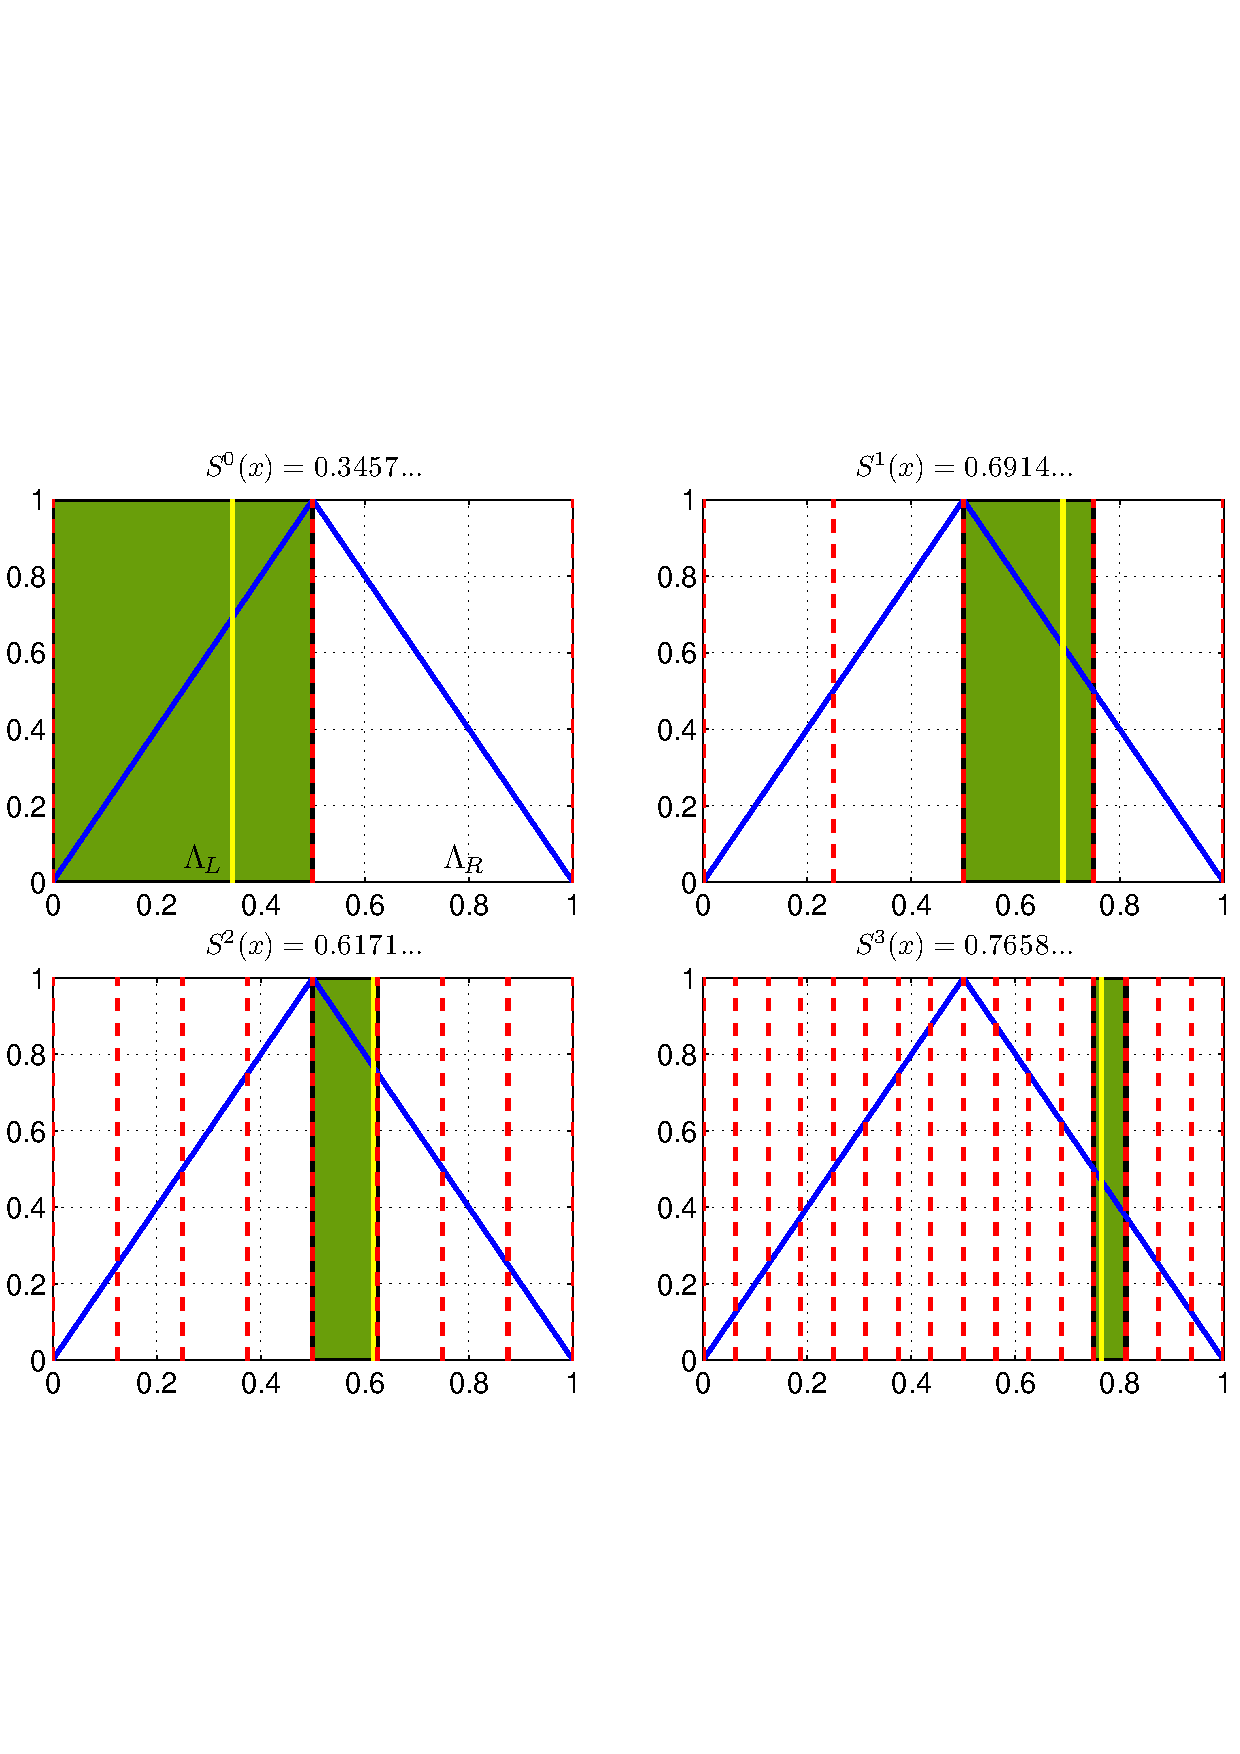
\includegraphics[width=0.7\textwidth]{tentmapplot2}
}
$x = 0.3457...  $, and $ \phi(x)=\{.LRRR...\}$.
%%%%%%%%%%%%%%%%%%%%%%%%%%%%%%%%%%%%%%%%%%%%%%%%%%%%%%%%%%%%%%%%%%%%%%%%%
%%%%%%%%%%%%%%%%%%%%%%%%%%%%%%%%%%%%%%%%%%%%%%%%%%%%%%%%%%%%%%%%%%%%%%%%%
\newpage
\oursection{Stochastic Symbol Sequence }
%%%%%%%%%%%%%%%%%%%%%%%%%%%%%%%%%%%%%%%%%%%%%%%%%%%%%%%%%%%%%%%%%%%%%%%%%
\begin{itemize}\setlength{\parskip}{0pt}  \setlength{\itemsep}{5pt} \setlength{\topsep}{0pt}
    \item Similar to symbolic dynamics, we want to use a sequence of numbers to represent a distribution in
          $\Omega \in L^{\infty}[\Lambda], \int_{\Lambda}dx=1 $.
\end{itemize}

\begin{definition} \textbf{Stochastic symbol sequence.}
Consider $\mathcal{S}$ to be the symbol list. Let $\Delta$ be the collection of all
semi-infinite sequences of elements in $[0,1]$. We define $\delta^\star \in \Delta$ for each
symbol $\star \in \mathcal{S}$ as
 \begin{align}
 \begin{split}
 \delta^\star &= \{.\delta_0^\star \delta_1^\star\cdots \delta_n^\star\cdots\} \\
 %\delta^R &= \{.\delta_0^R \delta_1^R\cdots \delta_n^R\cdots\}
 \end{split}
 \end{align}
with $\delta^\star_i \in [0,1]$ for all $i$.
\end{definition}
\begin{itemize}\setlength{\parskip}{0pt}  \setlength{\itemsep}{5pt} \setlength{\topsep}{0pt}
  \item $\sigma: \Delta \rightarrow \Delta $, shift operator
    $$\sigma(\delta^L)= \{.\delta^L_1\delta^L_2\cdots
           \delta^L_n\cdots\}$$
\end{itemize}
%%%%%%%%%%%%%%%%%%%%%%%%%%%%%%%%%%%%%%%%%%%%%%%%%%%%%%%%%%%%%%%%%%%%%%%%%
%%%%%%%%%%%%%%%%%%%%%%%%%%%%%%%%%%%%%%%%%%%%%%%%%%%%%%%%%%%%%%%%%%%%%%%%%
\newpage
\oursection{Stochastic Symbol Sequence }
%%%%%%%%%%%%%%%%%%%%%%%%%%%%%%%%%%%%%%%%%%%%%%%%%%%%%%%%%%%%%%%%%%%%%%%%%

\begin{itemize}\setlength{\parskip}{0pt}  \setlength{\itemsep}{5pt} \setlength{\topsep}{0pt}

    \item Consider $\mathcal{S} =\{L,R \}$, $\psi^L :\Omega \rightarrow \Delta$
               \begin{eqnarray}
               \label{psidef}
               %\delta^L_i = \int_{\Lambda_L} P^i_S \omega(x)dx \text{,   and  }
               \delta^L_i = \int_{\Lambda_L} P^i_S \left(\omega(x)\right)dx \text{, for all }i\ge0
               \end{eqnarray}
    \item For $x\in \Lambda$ having distribution $\omega$, the interpretation of $\delta_i^L$ is
             \begin{eqnarray}
             \label{deltaistar}
             \delta_i^L = \prob(\phi(x)_i = L) \text{, for } \text{ for all }i
              \end{eqnarray}


    \item If there are only two symbols $\mathcal{S} =\{L,R\}$, $\delta^R=1-\delta^L$.
    \item  Define $\psi \equiv \psi^L$, we have,
           \begin{lemma}
                $$\psi \circ P_S = \sigma \circ \psi$$
           \end{lemma}

\end{itemize}

   %\item  $\mathcal{S} = \{L,R\}$, $\delta_i^{L},\delta_i^{R} \in [0, 1]$,
   %        \begin{eqnarray}
   %        \delta^L = \{\cdots \delta_{-n}^L\cdots \delta_{-1}^L.\delta_0^L \delta_1^L\cdots \delta_n^L\cdots\} \nonumber\\
   %        \delta^R = \{\cdots \delta_{-n}^R\cdots \delta_{-1}^R.\delta_0^R \delta_1^R\cdots \delta_n^R\cdots\} \nonumber
   %        \end{eqnarray}

    %
    %$$\sigma(\delta^L)= \{\cdots \delta^L_{-n}\cdots \delta^L_{-1}\delta^L_0.\delta^L_1\cdots
    %       \delta^L_n\cdots\}$$

%%%%%%%%%%%%%%%%%%%%%%%%%%%%%%%%%%%%%%%%%%%%%%%%%%%%%%%%%%%%%%%%%%%%%%%%%
%%%%%%%%%%%%%%%%%%%%%%%%%%%%%%%%%%%%%%%%%%%%%%%%%%%%%%%%%%%%%%%%%%%%%%%%%
\newpage
\oursection{Stochastic Symbol Sequence }
%%%%%%%%%%%%%%%%%%%%%%%%%%%%%%%%%%%%%%%%%%%%%%%%%%%%%%%%%%%%%%%%%%%%%%%%%
\vspace{-0.7cm}
\begin{itemize}\setlength{\parskip}{0pt}  \setlength{\itemsep}{5pt} \setlength{\topsep}{0pt}
   \item Unfortunately, $\psi$ is not invertible. There are many $\omega\in \Omega$ which maps to the same $\delta$
   \item So we restrict $\omega$ to the following space,
         \vspace{-0.2cm}
        \begin{eqnarray}
        \label{DefOmegabar}
        \bar{\Omega} = \left\{ \omega \left| \omega(x) = \lim_{n \rightarrow \infty} \prod_{i=0}^n \beta^{\phi(x)_i}_i \right. \right\}
        \end{eqnarray}
        where $\beta^L_i \in [0,1]$, $\beta^R_i=1-\beta^L_i$.
         \vspace{-0.2cm}
         Then $\psi:\bar{\Omega} \rightarrow \Delta$ is invertible.
\end{itemize}
\begin{lemma} For $\omega \in \bar{\Omega}$, $\delta^L_i=\psi(\omega)_i = \beta^L_i$ for all $i$\end{lemma}
\vspace{0.5cm}
\begin{lemma} For $x \in \Lambda$ having pdf $\omega\in \bar{\Omega}$, and any $s^*\in \Sigma$, one has
         \begin{eqnarray*}
             \prob(\phi(x)_i=s_i^*) = 
             \prob(\phi(x)_i=s_i^* \mid  \phi(x)_k=s_k^*, \text{ for all } k \neq i )
          \\[-2cm]
          \end{eqnarray*}
\end{lemma}
This lemma says given $s_k$ does not help to know $s_i$. 



%%%%%%%%%%%%%%%%%%%%%%%%%%%%%%%%%%%%%%%%%%%%%%%%%%%%%%%%%%%%%%%%%%%%%%%%%
%%%%%%%%%%%%%%%%%%%%%%%%%%%%%%%%%%%%%%%%%%%%%%%%%%%%%%%%%%%%%%%%%%%%%%%%%
\newpage
\oursection{Stochastic Symbol Sequence }
%%%%%%%%%%%%%%%%%%%%%%%%%%%%%%%%%%%%%%%%%%%%%%%%%%%%%%%%%%%%%%%%%%%%%%%%%
\begin{itemize}\setlength{\parskip}{0pt}  \setlength{\itemsep}{5pt} \setlength{\topsep}{0pt}

   \item $P_S$ is the Perron-Frobenius operator of $S$
         \begin{eqnarray}
         P_S (\omega) \in \bar{\Omega}, \mbox{if } \omega \in \bar{\Omega} \nonumber
         \end{eqnarray}
   \item More importantly,
         \begin{eqnarray}
         P_S= \psi^{-1}\circ \sigma \circ \psi  \nonumber
         \end{eqnarray}
   \item Reminder: the above procedure is to find the subspace $\bar{\Omega}$ such that when $\omega\in\bar{\Omega}$, we can find $P_S^i(\omega)$ for all $i$ easily.
\end{itemize}
%%%%%%%%%%%%%%%%%%%%%%%%%%%%%%%%%%%%%%%%%%%%%%%%%%%%%%%%%%%%%%%%%%%%%%%%%
%%%%%%%%%%%%%%%%%%%%%%%%%%%%%%%%%%%%%%%%%%%%%%%%%%%%%%%%%%%%%%%%%%%%%%%%%
\newpage
\oursection{Total Variation Distance in $\bar{\Omega}$}
%%%%%%%%%%%%%%%%%%%%%%%%%%%%%%%%%%%%%%%%%%%%%%%%%%%%%%%%%%%%%%%%%%%%%%%%%
\begin{itemize}\setlength{\parskip}{0pt}  \setlength{\itemsep}{5pt} \setlength{\topsep}{0pt}
    \item $\omega$, $\hat{\omega}\in{\bar{\Omega}}$ have stochastic symbol sequences  $\{\delta^L, \delta^R\}$ and $\{\hat{\delta}^L,\hat{\delta}^R \}$, respectively.
          \begin{eqnarray}
            \label{infiniteTV}
            |\omega-\hat{\omega}|_{TV} = \frac{1}{2} \lim_{n \rightarrow \infty}  \sum_{s\in\Sigma} \left|
                                     \prod_{i=0}^n\delta_i^{s_i}-\prod_{i=0}^n\hat{\delta}_i^{s_i}  \right| \nonumber
          \end{eqnarray}
    \item $\delta_i^L = \hat{\delta}_i^L$ when $i\notin \theta$, and $|\theta| = p$.
          \begin{eqnarray}
           \label{finiteTV}
            |\omega-\hat{\omega}|_{TV} = \frac{1}{2} \sum_{s\in\Sigma_p}  \left|
                             \prod_{i\in \theta}\delta_i^{s_i}-\prod_{i\in\theta}\hat{\delta}_i^{s_i}  \right| \nonumber
          \end{eqnarray}
   where $\Sigma_p$ are all $(L,R)$ combinations of $p$ symbols($2^p$).
   %\item without loss of generality, assume $\delta^L_i =\delta^R_i$ for all $i$, and let $\delta \equiv \delta^L $
\end{itemize}

%%%%%%%%%%%%%%%%%%%%%%%%%%%%%%%%%%%%%%%%%%%%%%%%%%%%%%%%%%%%%%%%%%%%%%%%%
%%%%%%%%%%%%%%%%%%%%%%%%%%%%%%%%%%%%%%%%%%%%%%%%%%%%%%%%%%%%%%%%%%%%%%%%%
\newpage
\oursection{Total Variation Distance to Invariant Distribution}
%%%%%%%%%%%%%%%%%%%%%%%%%%%%%%%%%%%%%%%%%%%%%%%%%%%%%%%%%%%%%%%%%%%%%%%%%
\begin{itemize}\setlength{\parskip}{0pt}  \setlength{\itemsep}{5pt} \setlength{\topsep}{0pt}
    \item The invariant distribution of map $S$ is $\bar{\omega}$.
          $$\bar{\delta}\equiv \psi(\bar{\omega}) = \left\{.\frac{1}{2}\frac{1}{2}\frac{1}{2}...\right\}  $$
    \item $\omega \mapsto |\omega-\bar{\omega}|_{TV}$ is convex, so  $\delta \mapsto |\psi^{-1}(\delta)-\bar{\omega}|_{TV} $ is also convex.
    \item Using convexity, we can prove
          \begin{lemma}
          \label{alldifflemma}
           $\delta$ and $\hat{\delta}$ are two stochastic symbol sequences, each corresponds to the probability distribution $\omega$ and $\hat{\omega}$, respectively. Suppose there exists a bijection $\beta: i \mapsto j$ such that $|\delta_i-\frac{1}{2}| \ge |\hat{\delta}_j-\frac{1}{2} |$ for all $i\in \mathbb{Z}$, then
          \begin{eqnarray}
          |\omega-\bar{\omega} |_{TV} \ge|\hat{\omega}-\bar{\omega} |_{TV}
          \end{eqnarray}
\end{lemma}
\end{itemize}
%%%%%%%%%%%%%%%%%%%%%%%%%%%%%%%%%%%%%%%%%%%%%%%%%%%%%%%%%%%%%%%%%%%%%%%%%
%%%%%%%%%%%%%%%%%%%%%%%%%%%%%%%%%%%%%%%%%%%%%%%%%%%%%%%%%%%%%%%%%%%%%%%%%
\newpage
\oursection{Evaluate the Total Variation Distance}
%%%%%%%%%%%%%%%%%%%%%%%%%%%%%%%%%%%%%%%%%%%%%%%%%%%%%%%%%%%%%%%%%%%%%%%%%
\begin{itemize}\setlength{\parskip}{0pt}  \setlength{\itemsep}{0pt} \setlength{\topsep}{0pt}
\vspace{-1cm}
    \item Consider the flolowing two sequences
        \begin{eqnarray}
        \\[-1.5cm] \nonumber
         \hat{\delta} 
               = \{.\underbrace{\hat{\delta}_{\star} \hat{\delta}_{\star} \cdots \hat{\delta}_{\star}}_{p}\frac{1}{2}\frac{1}{2}\cdots\},  
         \bar{\delta}= \left\{.\frac{1}{2}\frac{1}{2}\frac{1}{2}\cdots\right\}\nonumber
        \\[-1.5cm] \nonumber
        \end{eqnarray}         
        %   $\hat{\delta}_0 =\hat{\delta}_1= \cdots = \hat{\delta}_{p-1}$
   \item The TV can be evaluated by finding the difference between two binomial distributions. %$|\psi^{-1}(\delta)-\psi^{-1}(\bar{\delta)}|^{TV}$
        \begin{eqnarray}
           |\hat{\omega}-\bar{\omega}|_{TV}
                     & = &\frac{1}{2} \sum_{s\in\Sigma_p}
                           \left| \prod_{i\in \theta}\hat{\delta}_i^{s_i}-\prod_{i\in\theta}\bar{\delta}_i^{s_i}  \right| \nonumber \\
                     & = &\frac{1}{2}  \sum_{k=0}^p {p \choose k}
                           \left|(\hat{\delta}_\star)^k (1-\hat{\delta}_\star)^{p-k} - \frac{1}{2^p} \right| \nonumber\\
                     & = &\frac{1}{2} \sum_{k=0}^p\left|\text{binomial}(k;p,\hat{\delta}_\star)-\text{binomial}\left(k;p,\frac{1}{2}\right)\right| \nonumber
     %                & \rightarrow &\erf \left( \sqrt{\frac{p}{2}}\left((\delta_{\star}^m)-\frac{1}{2}\right)\right) \text{, when } p\rightarrow \infty \text{, and } \delta_{\star}^m \rightarrow \frac{1}{2}
                    % & = &\frac{1}{2}  \sum_{k=0}^p \left|{p \choose k}
                    %       (\delta_\star)^k (1-\delta_\star)^{p-k} -{p \choose k} \frac{1}{2^p} \right|\nonumber
        \end{eqnarray}
\end{itemize}
%%%%%%%%%%%%%%%%%%%%%%%%%%%%%%%%%%%%%%%%%%%%%%%%%%%%%%%%%%%%%%%%%%%%%%%%%
%%%%%%%%%%%%%%%%%%%%%%%%%%%%%%%%%%%%%%%%%%%%%%%%%%%%%%%%%%%%%%%%%%%%%%%%%
\newpage
\oursection{Upper Bound and Lower Bound}
%%%%%%%%%%%%%%%%%%%%%%%%%%%%%%%%%%%%%%%%%%%%%%%%%%%%%%%%%%%%%%%%%%%%%%%%%
% the plot of ub,lb theorems
\begin{theorem}\textbf{Lower Bound.}
\label{theoremlb}
$\delta$ and $\bar{\delta}$ are two stochastic symbol sequences, each corresponds to the probability distribution $\omega$ and the invariant distribution $\bar{\omega}$, respectively. Suppose there is a set $\theta \subset \mathbb{Z}^++\{0\} $, $|\theta|=p$ such that for all $i \in \theta$, $|\delta_i-\frac{1}{2}|>\epsilon$, then
\begin{eqnarray}
\label{lbineq}
|\omega-\bar{\omega}|_{TV} \ge \mathbf{I}_{\frac{1}{2}}(p-k^*,k^*+1) - \mathbf{I}_{\frac{1}{2}-\epsilon}(p-k^*,k^*+1)
\end{eqnarray}
with
\begin{eqnarray}
\label{kstar}
k^* =  \left\lfloor p \frac{\log{2}+\log{(\frac{1}{2}-\epsilon)} }{\log{(\frac{1}{2}-\epsilon)}-\log{(\frac{1}{2}+\epsilon})} \right\rfloor
\end{eqnarray}
where $\mathbf{I}$ is the regularized incomplete beta function.
\end{theorem}
In this theorem, we bound $|\omega-\bar{\omega}|_{TV}$ by choosing $\hat{\delta}_\star = \frac{1}{2}+\epsilon$. 
%%%%%%%%%%%%%%%%%%%%%%%%%%%%%%%%%%%%%%%%%%%%%%%%%%%%%%%%%%%%%%%%%%%%%%%%%
%%%%%%%%%%%%%%%%%%%%%%%%%%%%%%%%%%%%%%%%%%%%%%%%%%%%%%%%%%%%%%%%%%%%%%%%%
\newpage
\oursection{The Limit of the Bounds}
%%%%%%%%%%%%%%%%%%%%%%%%%%%%%%%%%%%%%%%%%%%%%%%%%%%%%%%%%%%%%%%%%%%%%%%%%
%\begin{itemize}
%   \item
         \begin{align*}
         \hat{\delta}      = \{.\underbrace{\hat{\delta}_\star \hat{\delta}_\star \cdots \hat{\delta}_\star}_{p}\frac{1}{2}\frac{1}{2}\cdots\}, \,\,\,
         \bar{\delta}  = \left\{.\frac{1}{2}\frac{1}{2}\frac{1}{2}\cdots\right\}
         \end{align*}
%\end{itemize}
\begin{theorem}
\label{theoremapproxlb} $\bar{\omega}$ and $\hat{\omega}$ are two probability distributions, and have the stochastic
symbol sequences $\bar{\delta}$ and $\delta$ as defined above, respectively. Let $p
\rightarrow \infty$ and $\hat{\delta}_{\star} \rightarrow \frac{1}{2}$, then one has
\begin{align}
\begin{split}
  \label{lbublimit}
                 |\hat{\omega}-\bar{\omega}|_{TV}
               & =  \erf \left( \sqrt{\frac{p}{2}}\left((\hat{\delta}_{\star})-\frac{1}{2}\right)\right)
\end{split}
\end{align}


\end{theorem}


%%%%%%%%%%%%%%%%%%%%%%%%%%%%%%%%%%%%%%%%%%%%%%%%%%%%%%%%%%%%%%%%%%%%%%%%%
%%%%%%%%%%%%%%%%%%%%%%%%%%%%%%%%%%%%%%%%%%%%%%%%%%%%%%%%%%%%%%%%%%%%%%%%%
%\newpage
%\oursection{Moving and Reshaping}
%%%%%%%%%%%%%%%%%%%%%%%%%%%%%%%%%%%%%%%%%%%%%%%%%%%%%%%%%%%%%%%%%%%%%%%%%
%\centerline{
%\begin{tabular}{cc}
%\scalebox{1.1}[1.1]{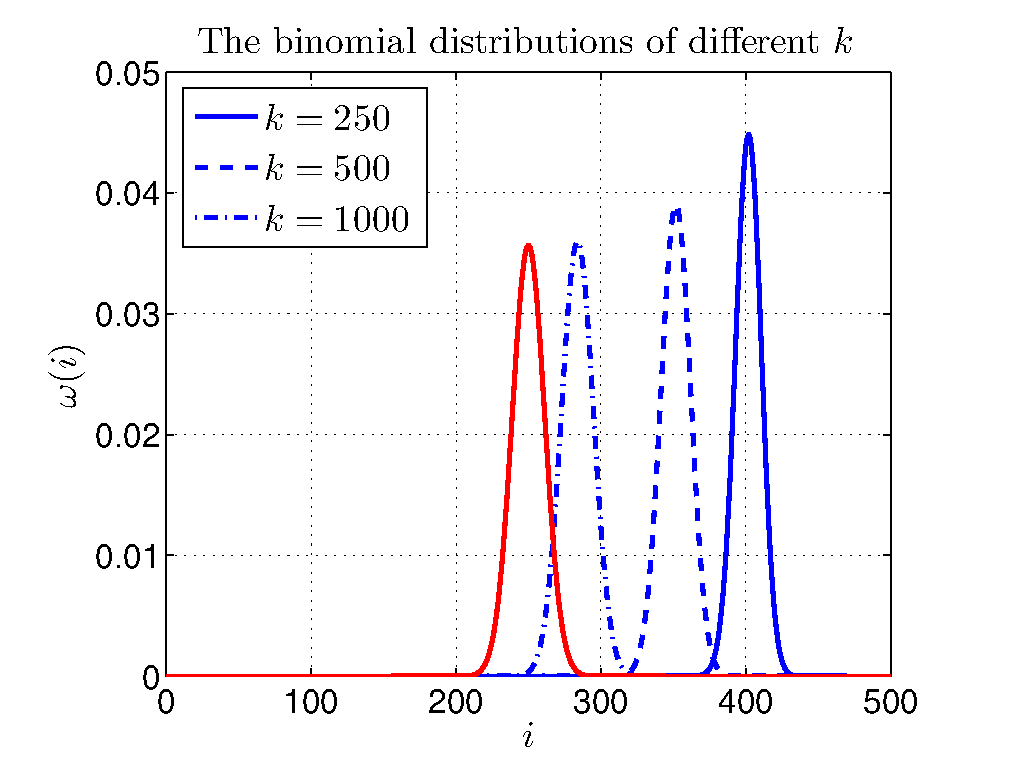
\includegraphics[width=0.38\textwidth,trim=0cm 0cm 0cm 0cm]{deltaMexample2a}}
%\scalebox{1.1}[1.1]{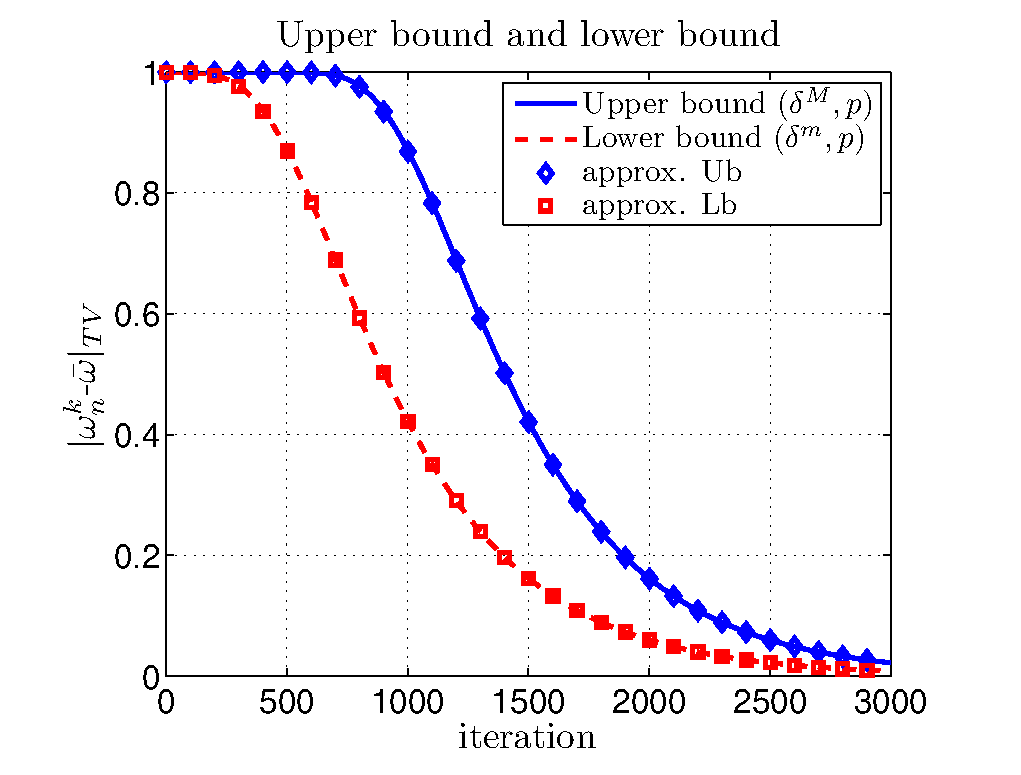
\includegraphics[width=0.38\textwidth,trim=0cm 0cm 0cm 0cm]{deltaMexample2b}} %\\
%\end{tabular}
%}
%\centerline{
%\scalebox{1.1}[1.1]{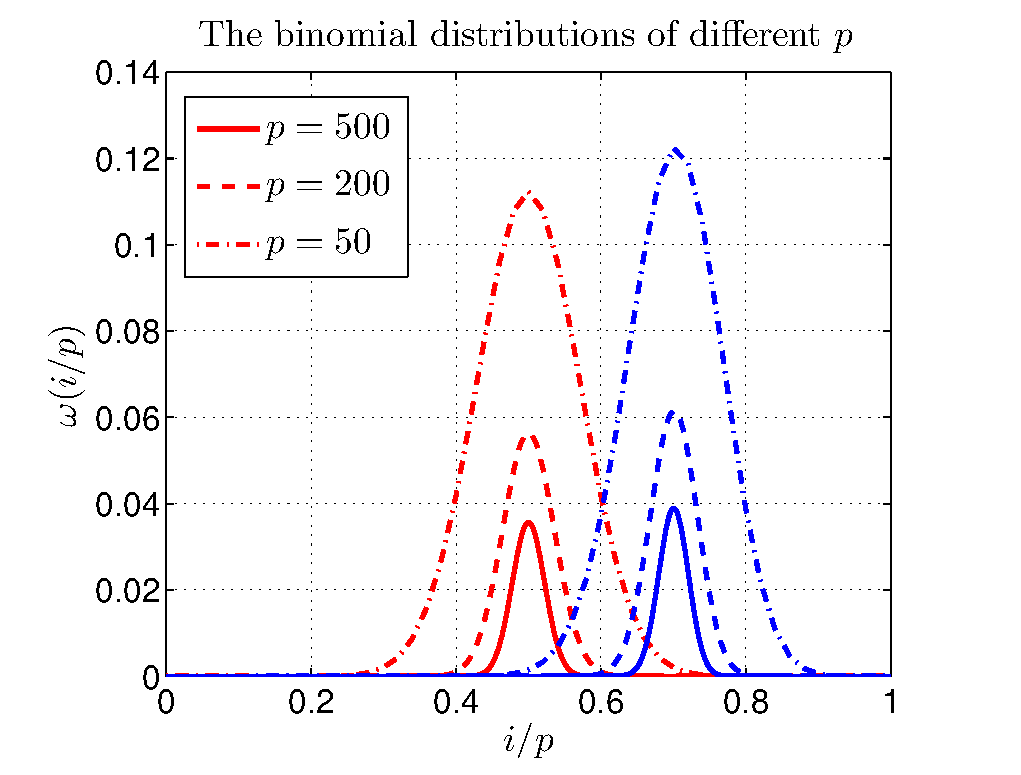
\includegraphics[width=0.38\textwidth,trim=0cm 0cm 0cm 0cm]{deltaMexample1a}}
%\scalebox{1.1}[1.1]{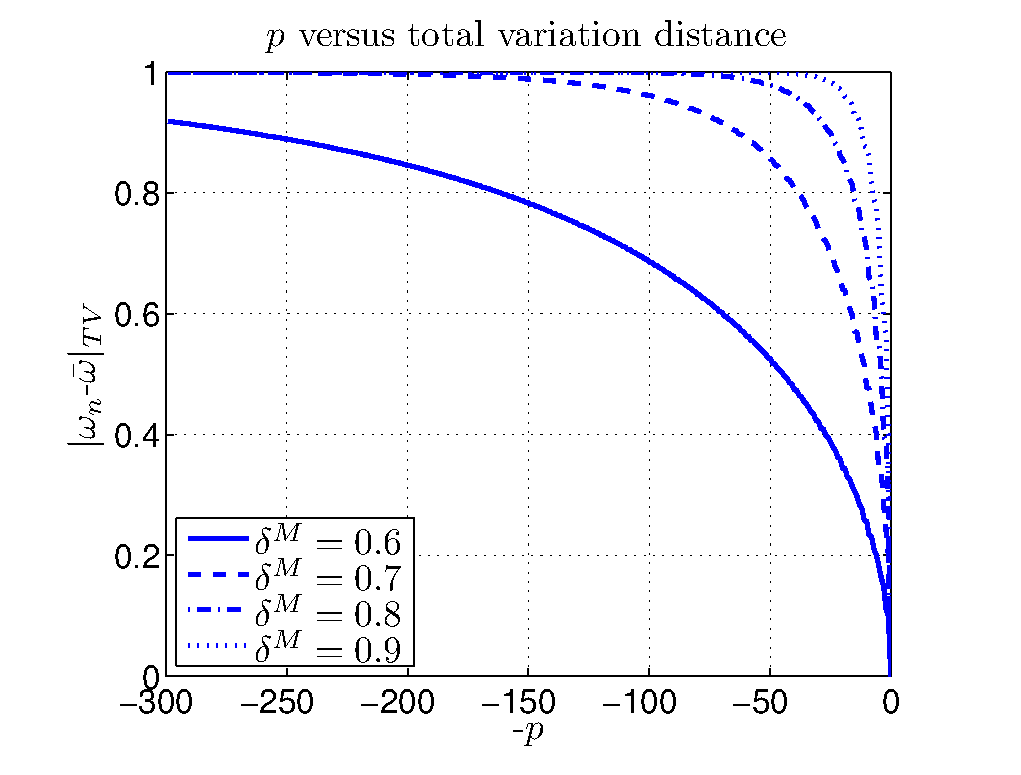
\includegraphics[width=0.38\textwidth,trim=0cm 0cm 0cm 0cm]{deltaMexample1b}}
%}
%%%%%%%%%%%%%%%%%%%%%%%%%%%%%%%%%%%%%%%%%%%%%%%%%%%%%%%%%%%%%%%%%%%%%%%%%
%%%%%%%%%%%%%%%%%%%%%%%%%%%%%%%%%%%%%%%%%%%%%%%%%%%%%%%%%%%%%%%%%%%%%%%%%
\newpage
\oursection{Create Cutoffs}
%%%%%%%%%%%%%%%%%%%%%%%%%%%%%%%%%%%%%%%%%%%%%%%%%%%%%%%%%%%%%%%%%%%%%%%%%
\begin{theorem}
Let $\omega_n^0 \in \bar{\Omega}$ has stochastic symbol sequence as the following,

\vspace{-1cm}

 \begin{eqnarray}
    \psi(\omega^0_n) =  \{.\delta_0 \delta_1 \delta_2 \cdots\}
 \end{eqnarray}
where $\delta_i = \min\{\frac{1}{2}+\epsilon_n r_n^i,1\}$, and
 \begin{align}
 %\begin{split}
   \epsilon_n = \sqrt{\frac{n(1-r_n)}{4}}, \,\,\,\,
            r_n = e^{-\frac{2}{n}}
 %\end{split}
 \end{align}
The family $(\Omega,\bar{\omega},(\omega^k_n)_{k=0,1,...})_{n=1,2,...}$ presents a Total Variation-cutoff. In fact,
Let $k = \frac{1}{4}n\log{n}+cn $, then for fixed $c\in \{-\infty,\infty\}$. as $n\rightarrow \infty$,
\begin{eqnarray}
\label{erfbound}
 %|\omega^k_n - \bar{\omega} |_{TV} \sim \erf \left(\frac{e^{-2c}}{\sqrt{8}}\right)
          \erf \left(\frac{e^{-2c-1}}{\sqrt{8}}\right)\le  |\omega^k_n - \bar{\omega} |_{TV} \le \erf \left(\frac{e^{-2c}}{\sqrt{8}}\right)
\end{eqnarray}
\end{theorem}

%%%%%%%%%%%%%%%%%%%%%%%%%%%%%%%%%%%%%%%%%%%%%%%%%%%%%%%%%%%%%%%%%%%%%%%%%
%%%%%%%%%%%%%%%%%%%%%%%%%%%%%%%%%%%%%%%%%%%%%%%%%%%%%%%%%%%%%%%%%%%%%%%%%
\newpage
\oursection{Conclusion}
%%%%%%%%%%%%%%%%%%%%%%%%%%%%%%%%%%%%%%%%%%%%%%%%%%%%%%%%%%%%%%%%%%%%%%%%%
\begin{itemize}

\item "It is believed that the cutoff phenomenon is widespread although it has only been proved for a rather small number of examples." - Laurent Saloff-Coste, Probability on Discrete Structures.
\item "To people studying finite Markov chains, the fact theorem 3.1 can be proved at all appears like a miracle." - Laurent Saloff-Coste, Probability on Discrete Structures.



%\item We successfully prove that one can generate a sequence of $\omega_n^0$ such that when they are evolved by any $1$-D chaotic map with symbolic dynamics, the family $(\Omega,\bar{\omega},(\omega^k_n)_{k=0,1,...})_{n=1,2,...}$ presents a Total Variation-cutoff, with desired cutoff time ($t_n$) and normal shape.
%\item We achieve this by
% \begin{enumerate}
%   \item Understanding what makes a cutoff with normal shapes.
%   \item Finding a subspace $\bar{\Omega}$ where we can evolve a probability distribution easily.
%   \item Bounding $\omega^k_n$ by binomial distributions in a further reduced space.
% \end{enumerate}


    %
\end{itemize}
%%%%%%%%%%%%%%%%%%%%%%%%%%%%%%%%%%%%%%%%%%%%%%%%%%%%%%%%%%%%%%%%%%%%%%%%%
%%%%%%%%%%%%%%%%%%%%%%%%%%%%%%%%%%%%%%%%%%%%%%%%%%%%%%%%%%%%%%%%%%%%%%%%%

%%%%%%%%%%%%%%%%%%%%%%%%%%%%%%%%%%%%%%%%%%%%%%%%%%%%%%%%%%%%%%%%%%%%%%%%%
%%%%%%%%%%%%%%%%%%%%%%%%%%%%%%%%%%%%%%%%%%%%%%%%%%%%%%%%%%%%%%%%%%%%%%%%%
%%%%%%%%%%%%%                 TOPIC a                          %%%%%%%%%%
%%%%%%%%%%%%%%%%%%%%%%%%%%%%%%%%%%%%%%%%%%%%%%%%%%%%%%%%%%%%%%%%%%%%%%%%%
%%%%%%%%%%%%%%%%%%%%%%%%%%%%%%%%%%%%%%%%%%%%%%%%%%%%%%%%%%%%%%%%%%%%%%%%%
\newpage
\oursection{\mytopica}
   \begin{itemize}
      \item Microfluidics and the Mixing Problem
      \item How chaotic mixing works?
      \item Forming the optimization problem
     % \item Finding a decent direction
      \item Methods and Tools 
      \item Results
   \end{itemize}


%%%%%%%%%%%%%%%%%%%%%%%%%%%%%%%%%%%%%%%%%%%%%%%%%%%%%%%%%%%%%%%%%%%%%%%%%
%%%%%%%%%%%%%%%%%%%%%%%%%%%%%%%%%%%%%%%%%%%%%%%%%%%%%%%%%%%%%%%%%%%%%%%%%
\newpage
\oursection{Microfluidics and the Mixing Problem}
%%%%%%%%%%%%%%%%%%%%%%%%%%%%%%%%%%%%%%%%%%%%%%%%%%%%%%%%%%%%%%%%%%%%%%%%%
\begin{itemize}
\item Microfluidic systems control and manipulate liquids in microliter or nanoliter scale.
\item Microfluidic mixing channel: objective is to mix two different liquids thoroughly.
\item Reynolds number $\text{Re} = \frac{Ul}{\nu}\approx 1$: flow is laminar.  P\'{e}clet number $\text{Pe} = \frac{Ul}{D} \gg 1$: diffusion is slow comparing with convection.
\item For example: $\text{Pe}=10^5$, the length of a smooth channel required for mixing is $10^3\,\text{cm}$. It grows linearly with $\text{Pe}$.
\item Chaotic mixing protocols is suggested in the design of mixing channel, and believed to have the best mixing.
\end{itemize}


%%%%%%%%%%%%%%%%%%%%%%%%%%%%%%%%%%%%%%%%%%%%%%%%%%%%%%%%%%%%%%%%%%%%%%%%%
\newpage
\begin{example}{\bfseries Stroock's Harringbone-type Mixer}
%%%%%%%%%%%%%%%%%%%%%%%%%%%%%%%%%%%%%%%%%%%%%%%%%%%%%%%%%%%%%%%%%%%%%%%%%
%%%%%%%%%%%%%%%%%%%%%%%%%%%%%%%%%%%%%%%%%%%%%%%%%%%%%%%%%%%%%%%%%%%%%%%%%
  \begin{figure}
    \centerline{
       \scalebox{0.3}[0.3]{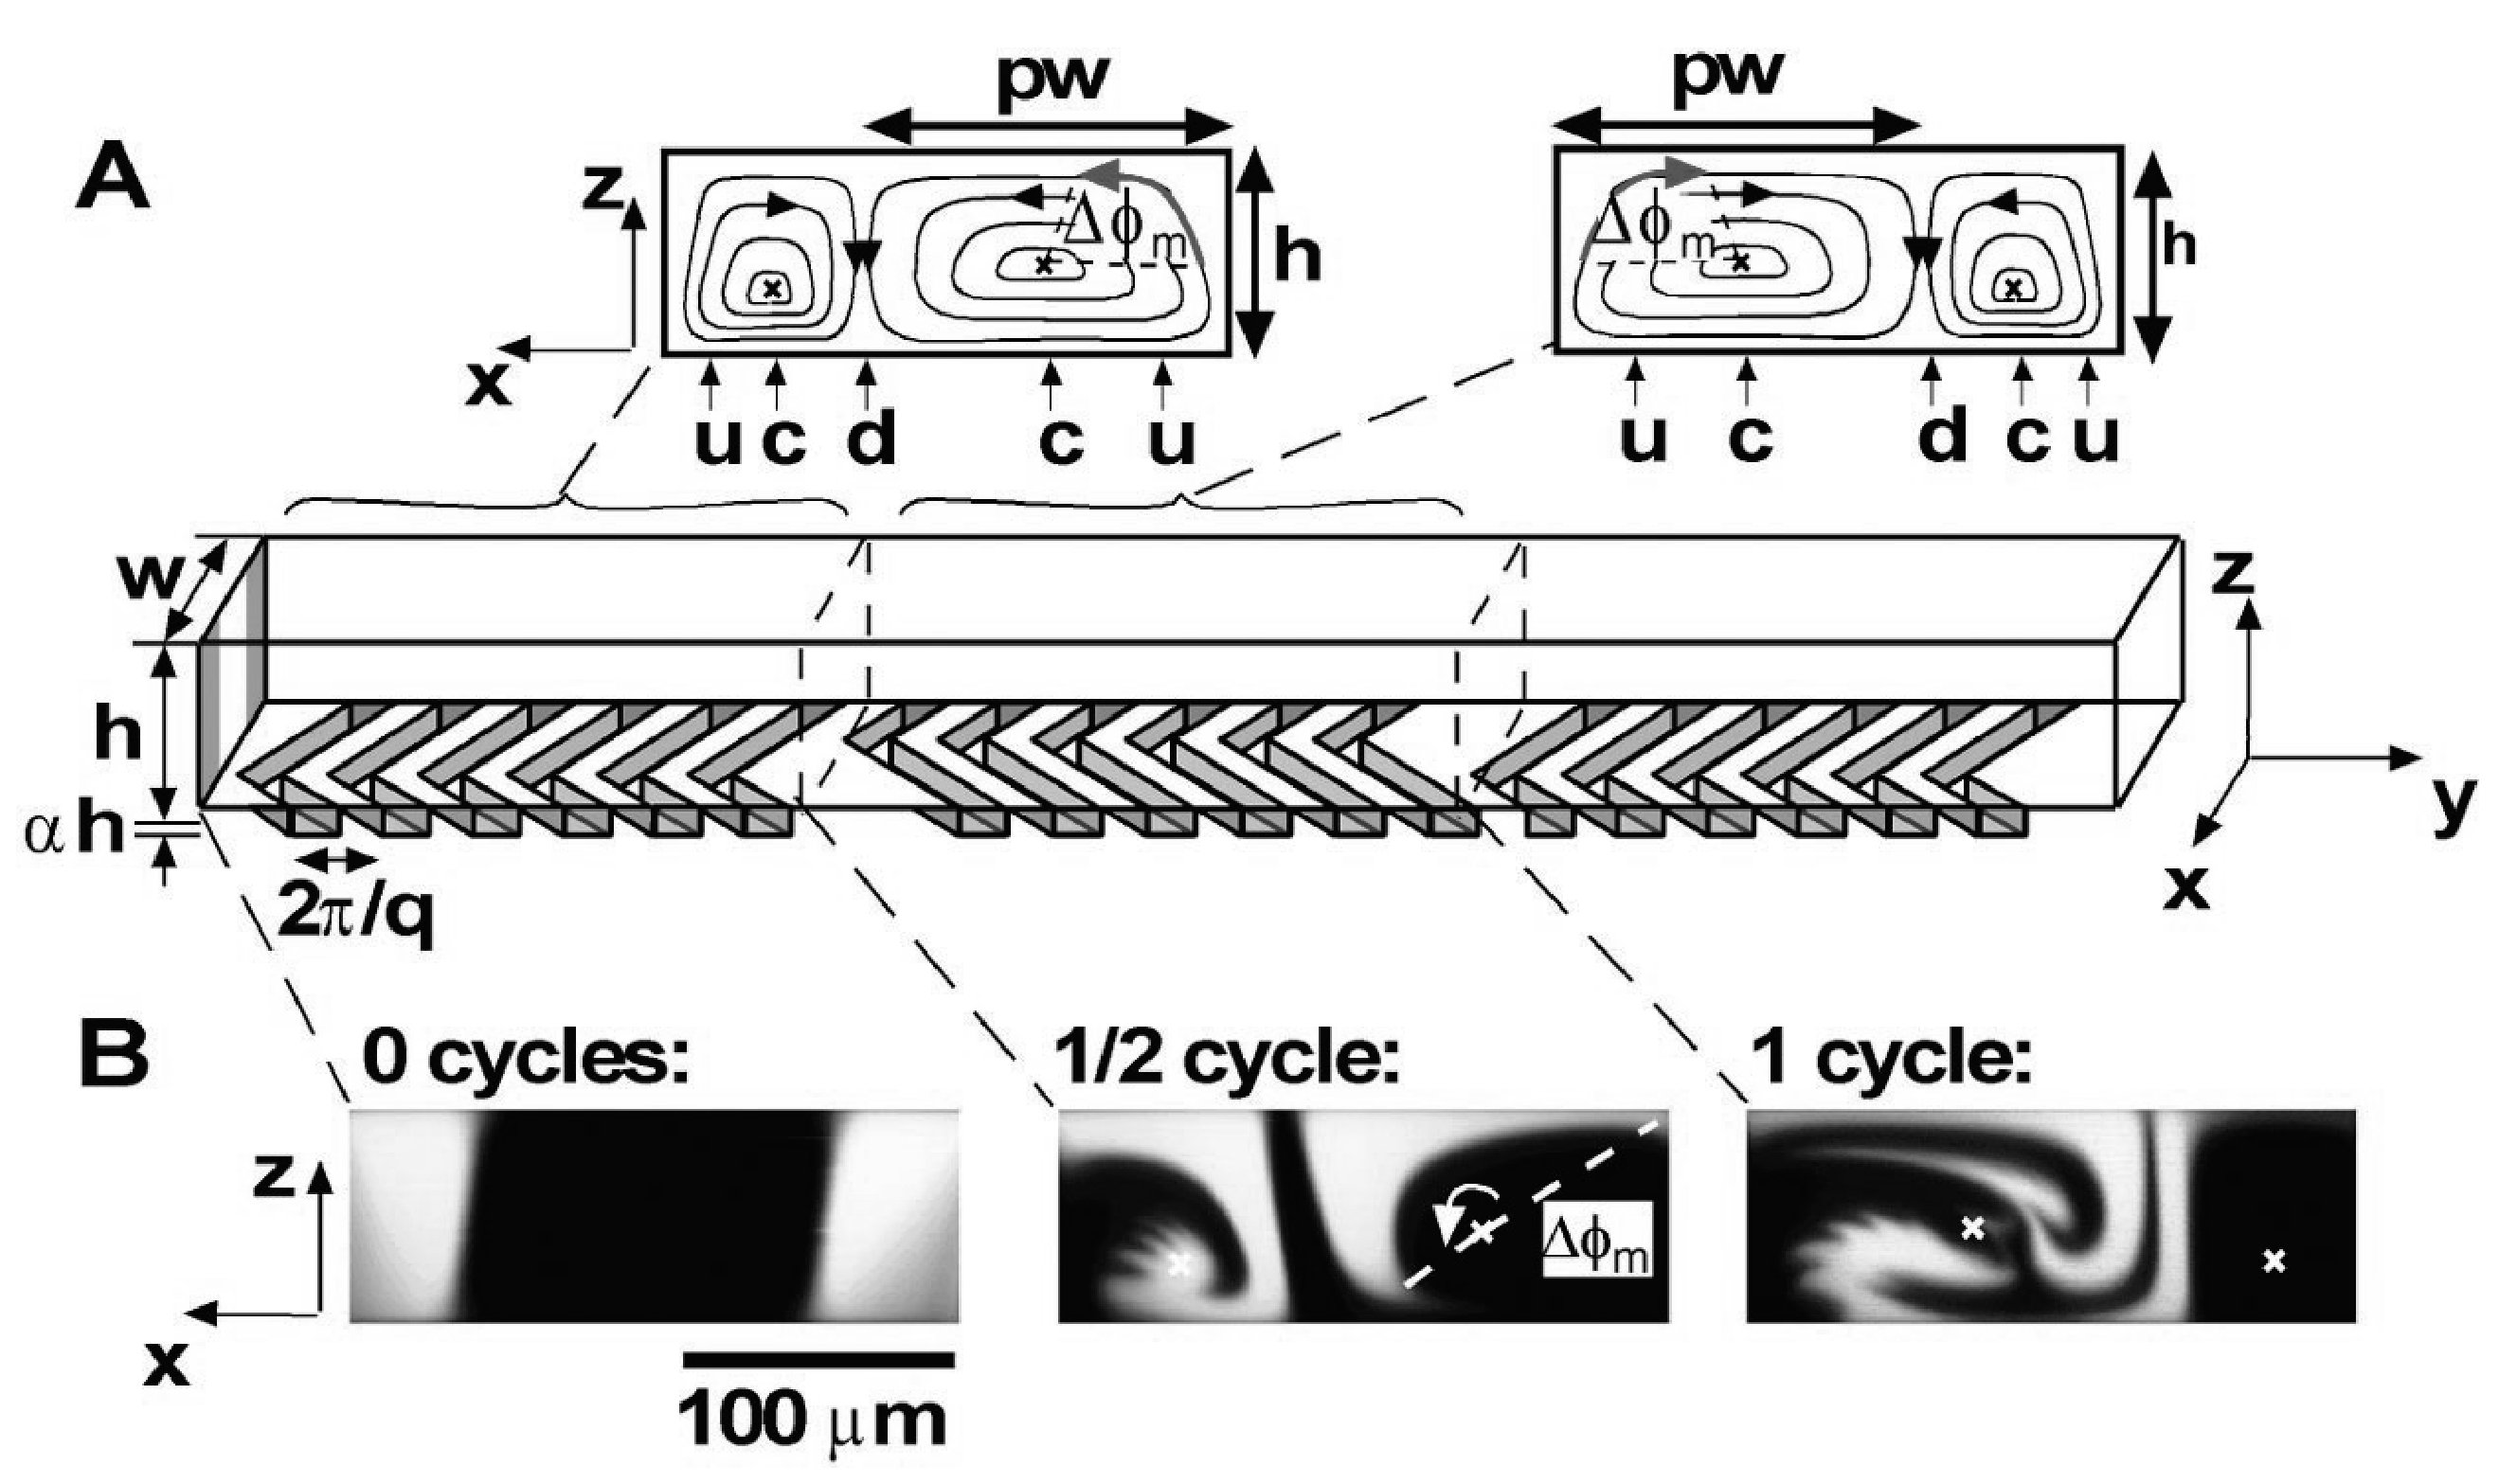
\includegraphics{stroockmixer}}
       \scalebox{0.8}[0.8]{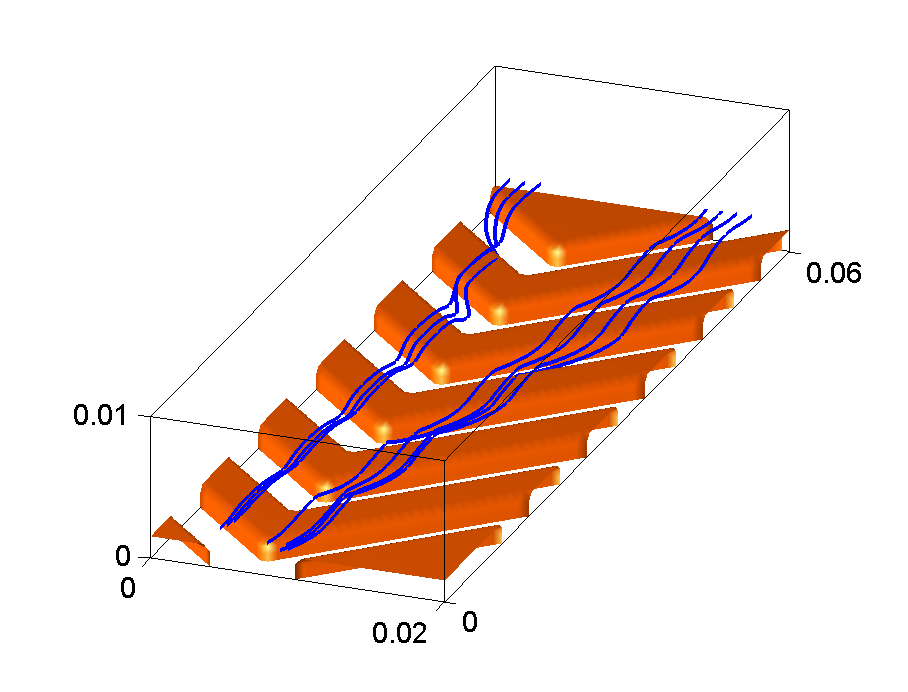
\includegraphics{stroockstructure}}
    }
  \end{figure}
\begin{itemize}\setlength{\parskip}{0pt}  \setlength{\itemsep}{10pt} \setlength{\topsep}{0pt}
\item Abrahan D. Stroock, et. al. Chaotic Mixer for Microchannels. Science. 2002. 
\item Mixing length grows linearly with $\log(\text{Pe})$ 
\end{itemize}
\end{example}

%%%%%%%%%%%%%%%%%%%%%%%%%%%%%%%%%%%%%%%%%%%%%%%%%%%%%%%%%%%%%%%%%%%%%%%%%
\newpage
\oursection{How chaotic mixing works?}
%%%%%%%%%%%%%%%%%%%%%%%%%%%%%%%%%%%%%%%%%%%%%%%%%%%%%%%%%%%%%%%%%%%%%%%%%
%%%%%%%%%%%%%%%%%%%%%%%%%%%%%%%%%%%%%%%%%%%%%%%%%%%%%%%%%%%%%%%%%%%%%%%%%
\vspace{-0.8cm}
  \begin{figure}
    \centerline{
       \scalebox{0.74}[0.74]{\includegraphics{chaoticmixing}}
    }
  \end{figure}

%%%%%%%%%%%%%%%%%%%%%%%%%%%%%%%%%%%%%%%%%%%%%%%%%%%%%%%%%%%%%%%%%%%%%%%%%
\newpage
\oursection{Problem Statement}
%%%%%%%%%%%%%%%%%%%%%%%%%%%%%%%%%%%%%%%%%%%%%%%%%%%%%%%%%%%%%%%%%%%%%%%%%
%%%%%%%%%%%%%%%%%%%%%%%%%%%%%%%%%%%%%%%%%%%%%%%%%%%%%%%%%%%%%%%%%%%%%%%%%
\centerline{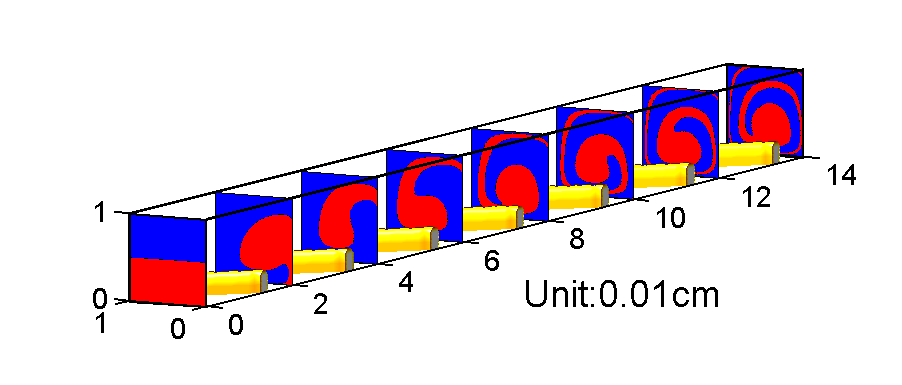
\includegraphics[width=0.6\textwidth]{mixingchannel}}
\begin{itemize}\setlength{\parskip}{0pt}  \setlength{\itemsep}{10pt} \setlength{\topsep}{0pt}
\item Our Goal: Improve Stroock's harringbone-type mixer.
\item Objective function: A linear function of velocity.
\item Design parameter: Material distribution inside the channel.
\item Assumptions: Flow is laminar, and driven by a constant body force.  The velocity field is fully developed. Both the structure and the velocity are periodical.
\end{itemize}
%%%%%%%%%%%%%%%%%%%%%%%%%%%%%%%%%%%%%%%%%%%%%%%%%%%%%%%%%%%%%%%%%%%%%%%%%
%%%%%%%%%%%%%%%%%%%%%%%%%%%%%%%%%%%%%%%%%%%%%%%%%%%%%%%%%%%%%%%%%%%%%%%%%
%\newpage
%\oursection{Problem Statement}
%\centerline{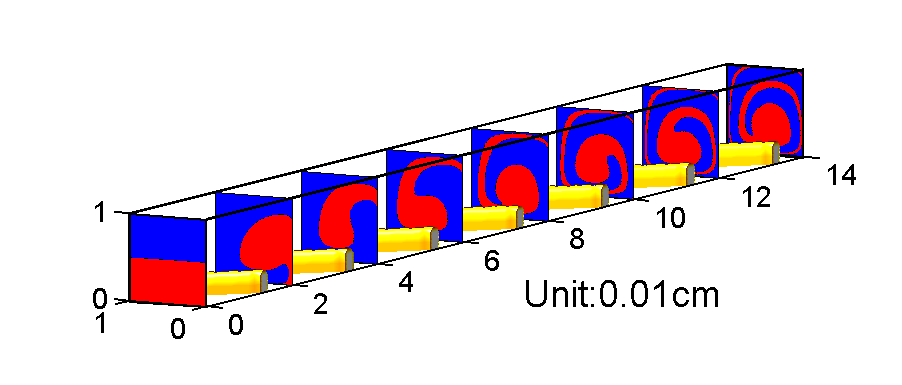
\includegraphics[width=0.6\textwidth,trim=1cm 2cm 0cm 3cm,clip]{mixingchannel}}
%\centerline{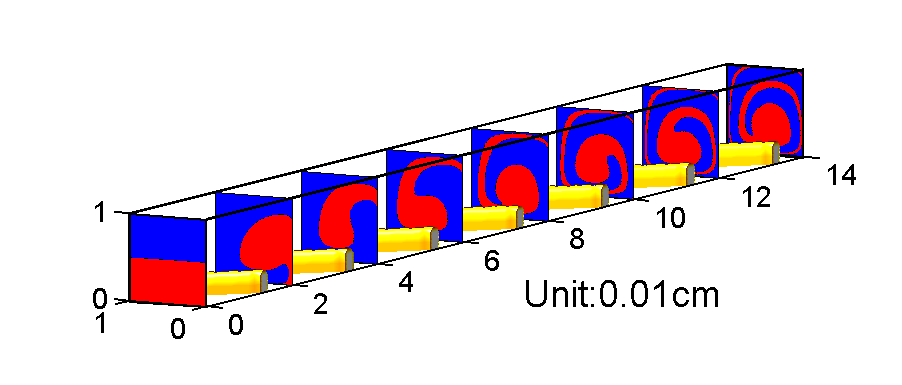
\includegraphics[width=0.6\textwidth]{mixingchannel}}

%\begin{itemize}
%\setlength{\topsep}{0cm}\setlength{\parskip}{0cm}\setlength{\parsep}{0cm}\setlength{\itemsep}{0cm}
%\item Goal: design and optimize a passive mixing channel which mixes two separated liquids in short length and microfluidic scale.
%\item Use internal structures to stir the flow and produce transverse velocity to enhance the mixing.
%\item Flow is laminar, and driven by a constant body force.  The velocity field is fully developed. Both the structure and the velocity are periodical.
%\end{itemize}
%%%%%%%%%%%%%%%%%%%%%%%%%%%%%%%%%%%%%%%%%%%%%%%%%%%%%%%%%%%%%%%%%%%%%%%%%
%%%%%%%%%%%%%%%%%%%%%%%%%%%%%%%%%%%%%%%%%%%%%%%%%%%%%%%%%%%%%%%%%%%%%%%%%
%\newpage
%\oursection{Challenges}
%\vspace{-0.5cm}
%\begin{itemize}
%  \item{Phyiscally}
%  \begin{itemize}\setlength{\parskip}{0pt}  \setlength{\itemsep}{5pt} \setlength{\topsep}{0pt}
%   \item Reynolds number $\text{Re} = \frac{Ul}{\nu}\approx 1$: flow is laminar
%   \item P\'{e}clet number $\text{Pe} = \frac{Ul}{D} \gg 1$: diffusion is slow comparing with convection
%  \end{itemize}
%\end{itemize}
%\begin{eqnarray*}
%\begin{aligned}
%  U  &:\text{ average flow velocity}(1\,\text{cm}\,\text{s}^{-1}),\\
%  l  &:\text{ characteristic length}(0.01 \,\text{cm}), \\
%  \nu&:\text{ kinematic viscosity}(0.01\,\text{g}\,\text{cm}^{-1}\,\text{s}^{-1}), \\
%  D  &:\text{ molecular diffusivity}(10^{-6} \,\text{cm}^2\,\text{s}^{-1}).
%\end{aligned}
%\end{eqnarray*}
%%%%%%%%%%%%%%%%%%%%%%%%%%%%%%%%%%%%%%%%%%%%%%%%%%%%%%%%%%%%%%%%%%%%%%%%%
%%%%%%%%%%%%%%%%%%%%%%%%%%%%%%%%%%%%%%%%%%%%%%%%%%%%%%%%%%%%%%%%%%%%%%%%%
\newpage
\oursection{Topology Optimization}
\begin{itemize}
  \item A typical topology optimization problem is to distribute a given amount of material in a design domain subject to load and support conditions such that the stiffness of the structure is maximized.
  \item No initial knowledge about the structure.
  \item When applying to the mixing channel design,
  \begin{itemize}\setlength{\parskip}{0pt}  \setlength{\itemsep}{5pt} \setlength{\topsep}{0pt}
    \item A large problem ($n_x=100, n_y=n_z=50$: over $10^6$ variables.)
    \item Nonlinear(nonconvex) optimization.
    %\item No clear defined measure of mixing.
    %\item No clear way to realize the Linked Twist Map (LTM) design procedure.
  \end{itemize}
\end{itemize}



%%%%%%%%%%%%%%%%%%%%%%%%%%%%%%%%%%%%%%%%%%%%%%%%%%%%%%%%%%%%%%%%%%%%%%%%%
%%%%%%%%%%%%%%%%%%%%%%%%%%%%%%%%%%%%%%%%%%%%%%%%%%%%%%%%%%%%%%%%%%%%%%%%%
\newpage
\oursection{Stokes Equation and Darcey Flow}

\begin{itemize}
\item Generalized Stokes partial differential equation for imcompressible flow (Darcey equation)
       \begin{eqnarray*}
       ( -\nu\Delta + \mathbf{\alpha} \mathbf{I}) \mathbf{u} +\nabla  \mathbf{p} & = & \mathbf{f}\\
       \text{div} \mathbf{u}& = & 0
       \end{eqnarray*}

       $\mathbf{u}$: velocity, $\mathbf{p}$: pressure, $\mathbf{f}$: body force and boundary conditions
       $\nu$: kinematic viscosity, and $\bf{\alpha}$: inverse permeability
\item Discrete version
       \begin{equation}
       \left[\begin{matrix}
       -\nu \mathbf{L} + \mathbf{H} \mathbf{\bar{\alpha}}  & \mathbf{G}\\
       \mathbf{D}               &  0
       \end{matrix} \right]
    \left[\begin{matrix}
    \mathbf{\bar{u}} \\ \mathbf{\bar{p}}
    \end{matrix} \right]=
    \left[\begin{matrix}
    \mathbf{\bar{f}} \\ \mathbf{0}
    \end{matrix} \right]
    \end{equation}
\end{itemize}

%%%%%%%%%%%%%%%%%%%%%%%%%%%%%%%%%%%%%%%%%%%%%%%%%%%%%%%%%%%%%%%%%%%%%%%%%
%%%%%%%%%%%%%%%%%%%%%%%%%%%%%%%%%%%%%%%%%%%%%%%%%%%%%%%%%%%%%%%%%%%%%%%%%
\newpage
\oursection{Forming the optimization problem}
Topology optimization problem:
\begin{align*}
  \mbox{minimize     } & \,\,g(\mathbf{\bar{u}},\mathbf{\bar{p}},\mathbf{\bar{\alpha}}) \\
  \mbox{s.t.       }&
    \left[\begin{matrix}
     -\nu \mathbf{L} + \mathbf{H} \mathbf{\bar{\alpha}}  & \mathbf{G}\\
      \mathbf{D}               &  0
    \end{matrix} \right]
    \left[\begin{matrix}
      \mathbf{\bar{u}} \\ \mathbf{\bar{p}}
    \end{matrix} \right]=
    \left[\begin{matrix}
     \mathbf{\bar{f}} \\ \mathbf{0}
    \end{matrix} \right] \\
  & \mathbf{0}\le \mathbf{\bar{\alpha}} \le \alpha_M\mathbf{1}\\
\intertext{Lump the equality constraints into the objective function:}
   \mbox{minimize   }  & \,\,g(\mathbf{\bar{u}(\mathbf{\bar{\alpha}})},\mathbf{\bar{p}(\mathbf{\bar{\alpha}})},\mathbf{\bar{\alpha}}) \\
   \mbox{s.t.    } & \mathbf{0}\le \mathbf{\bar{\alpha}} \le \alpha_M\mathbf{1}
\end{align*}

%%%%%%%%%%%%%%%%%%%%%%%%%%%%%%%%%%%%%%%%%%%%%%%%%%%%%%%%%%%%%%%%%%%%%%%%%
%%%%%%%%%%%%%%%%%%%%%%%%%%%%%%%%%%%%%%%%%%%%%%%%%%%%%%%%%%%%%%%%%%%%%%%%%
%\newpage
%\oursection{The Objective Functions and the Simulation}
%The Objective Functions
%\begin{itemize}
%\vspace{-0.3cm}
%\setlength{\topsep}{0cm}\setlength{\parskip}{0cm}\setlength{\parsep}{0cm}\setlength{\itemsep}{0cm}
%\item A linear function of velocity
%\item A measure of the difference between the current flow map and the desired flow map.
%\end{itemize}
%\vspace{-0.5cm}
%The Simulation
%\begin{itemize}
%\vspace{-0.3cm}
%\setlength{\topsep}{0cm}\setlength{\parskip}{0cm}\setlength{\parsep}{0cm}\setlength{\itemsep}{0cm}
%\item Develop a probabilistic model based on optimal model reduction to approximate the solution of advection-diffusion equation on the cross-sections of the channel.
%      \begin{eqnarray*}
%       \frac{\partial \phi}{\partial t} + \mathbf{u} \cdot \nabla \phi = D \Delta \phi
%      \end{eqnarray*}
%where $\phi$ is the color intensity, and $\mathbf{u}$ the velocity field.
%\end{itemize}


%%%%%%%%%%%%%%%%%%%%%%%%%%%%%%%%%%%%%%%%%%%%%%%%%%%%%%%%%%%%%%%%%%%%%%%%%
%%%%%%%%%%%%%%%%%%%%%%%%%%%%%%%%%%%%%%%%%%%%%%%%%%%%%%%%%%%%%%%%%%%%%%%%%
%\newpage
%\oursection{With and Without Diffusion}
%\centerline{
%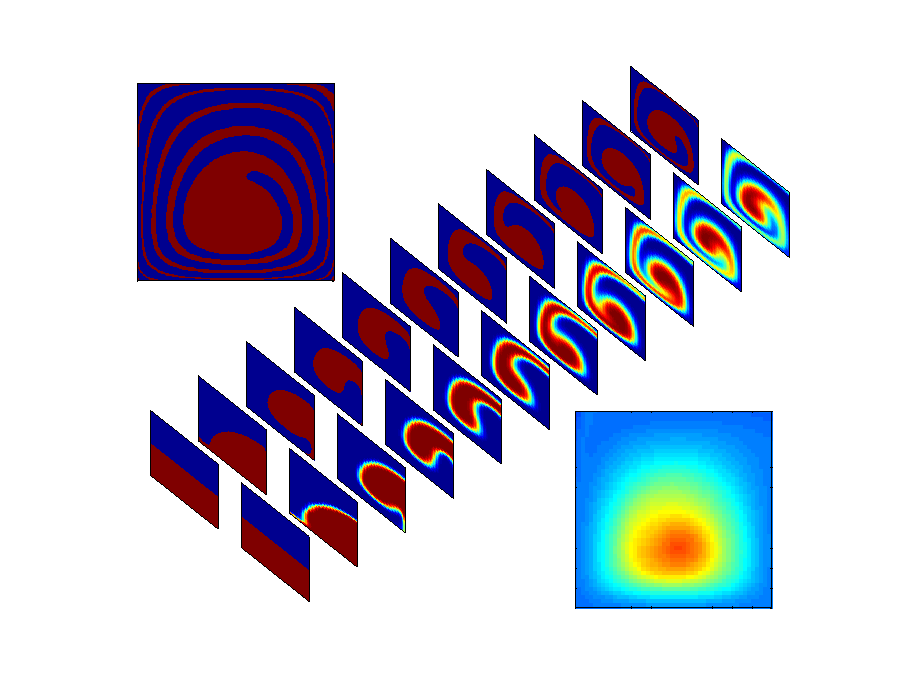
\includegraphics[width=0.8\textwidth,trim=0cm 1cm 0cm 0.5cm,clip]{markovvsexact}
%}
%%%%%%%%%%%%%%%%%%%%%%%%%%%%%%%%%%%%%%%%%%%%%%%%%%%%%%%%%%%%%%%%%%%%%%%%%
%%%%%%%%%%%%%%%%%%%%%%%%%%%%%%%%%%%%%%%%%%%%%%%%%%%%%%%%%%%%%%%%%%%%%%%%%
%\newpage
%\oursection{The Map Defined by Streamlines}
%\begin{tabular}{rl}
%\includegraphics[width=0.5\textwidth,trim=1cm 1cm 0cm 0cm]{computedmixingchannel}&
%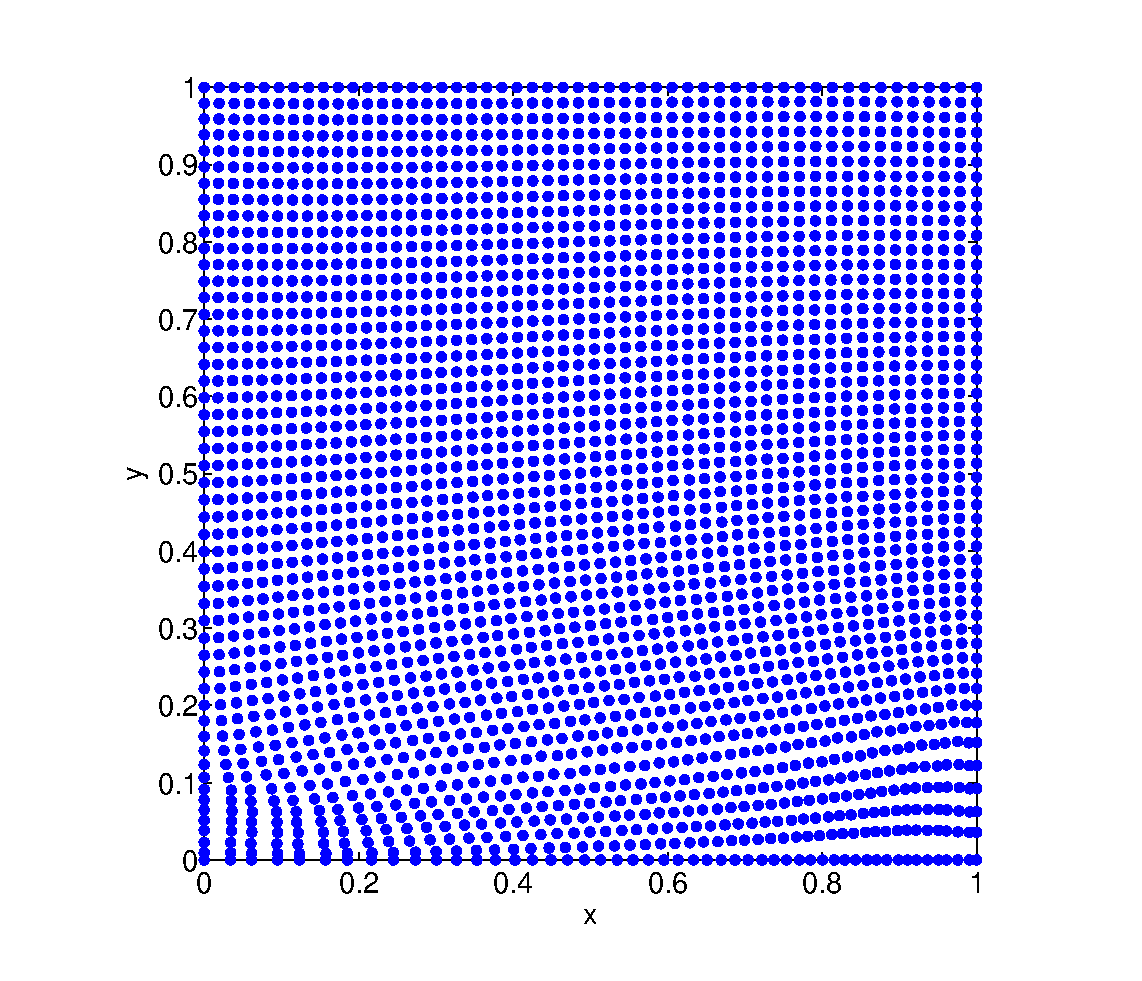
\includegraphics[width=0.5\textwidth,trim=1cm 1cm 0cm 0cm]{mappedpoints}
%\end{tabular}

%%%%%%%%%%%%%%%%%%%%%%%%%%%%%%%%%%%%%%%%%%%%%%%%%%%%%%%%%%%%%%%%%%%%%%%%%
%%%%%%%%%%%%%%%%%%%%%%%%%%%%%%%%%%%%%%%%%%%%%%%%%%%%%%%%%%%%%%%%%%%%%%%%%
\newpage
\oursection{Methods and Tools}
%%%%%%%%%%%%%%%%%%%%%%%%%%%%%%%%%%%%%%%%%%%%%%%%%%%%%%%%%%%%%%%%%%%%%%%%%
Methods
\vspace{-0.8cm}
\begin{itemize}\setlength{\parskip}{0pt}  \setlength{\itemsep}{10pt} \setlength{\topsep}{0pt}
\item Finite difference method with staggered mesh to solve the flow field.
\item Second order Runge-Kutta method to integrate streamlines.
\item Adjoint method to find $\frac{dg}{d\bar{\alpha}}$ without forming $\frac{d\bar{u}}{d\bar{\alpha}}$.
\item A gradient-based optimization scheme with fixed step size.
\item A probabilistic model to approximate the solution of the Advection-Diffusion equation on the cross-sections of the channel.
\end{itemize}
\vspace{-0.6cm}
Tools
\vspace{-0.8cm}
\begin{itemize}\setlength{\parskip}{0pt}  \setlength{\itemsep}{10pt} \setlength{\topsep}{0pt}
\item PETSc(Portable, Extensible Toolkit for Scientific Computation)
%\item Develope a package that communicates PETSc and Matlab
\item A 72-node PC cluster. 1G bytes memory for each CPU and gigabytes intranet connection.
\end{itemize}





%\item Eigenvector and eigenvalues: SLEPc(Scalable Library for Eigenvalue Problem Computations)
%\item FFT: FFTW(Fastest Fourier Transform in the West)

%%%%%%%%%%%%%%%%%%%%%%%%%%%%%%%%%%%%%%%%%%%%%%%%%%%%%%%%%%%%%%%%%%%%%%%%%
%\newpage
%\oursection{Results}
%%%%%%%%%%%%%%%%%%%%%%%%%%%%%%%%%%%%%%%%%%%%%%%%%%%%%%%%%%%%%%%%%%%%%%%%%
%%%%%%%%%%%%%%%%%%%%%%%%%%%%%%%%%%%%%%%%%%%%%%%%%%%%%%%%%%%%%%%%%%%%%%%%%
%\begin{example}{\bfseries Maximize the downward velocity at the center of the channel}
%  \begin{figure}
%    \centerline{
%       \scalebox{0.8}[0.8]{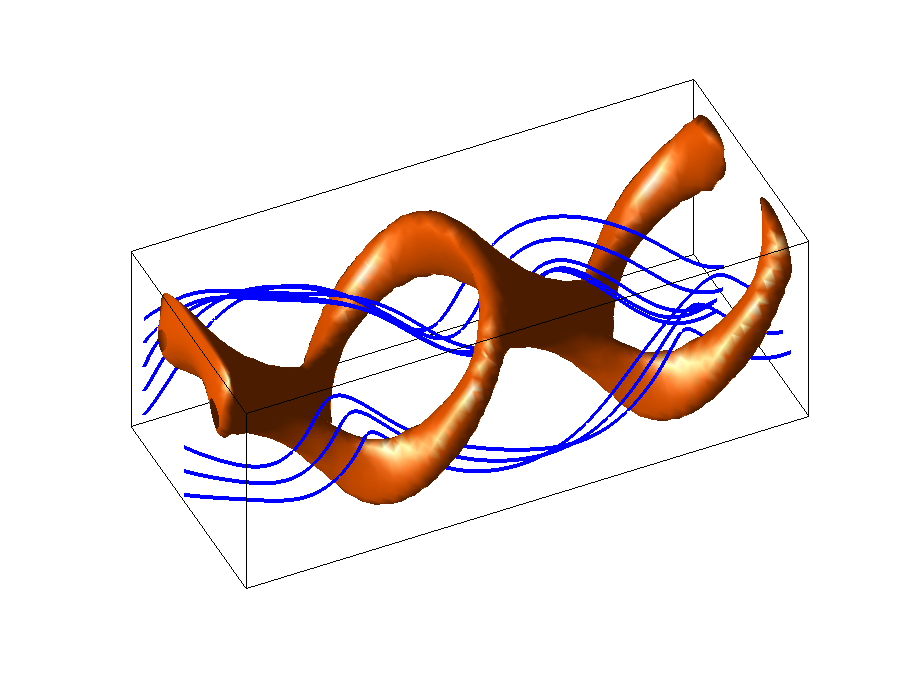
\includegraphics{example1structure2}}
%       \scalebox{0.7}[0.7]{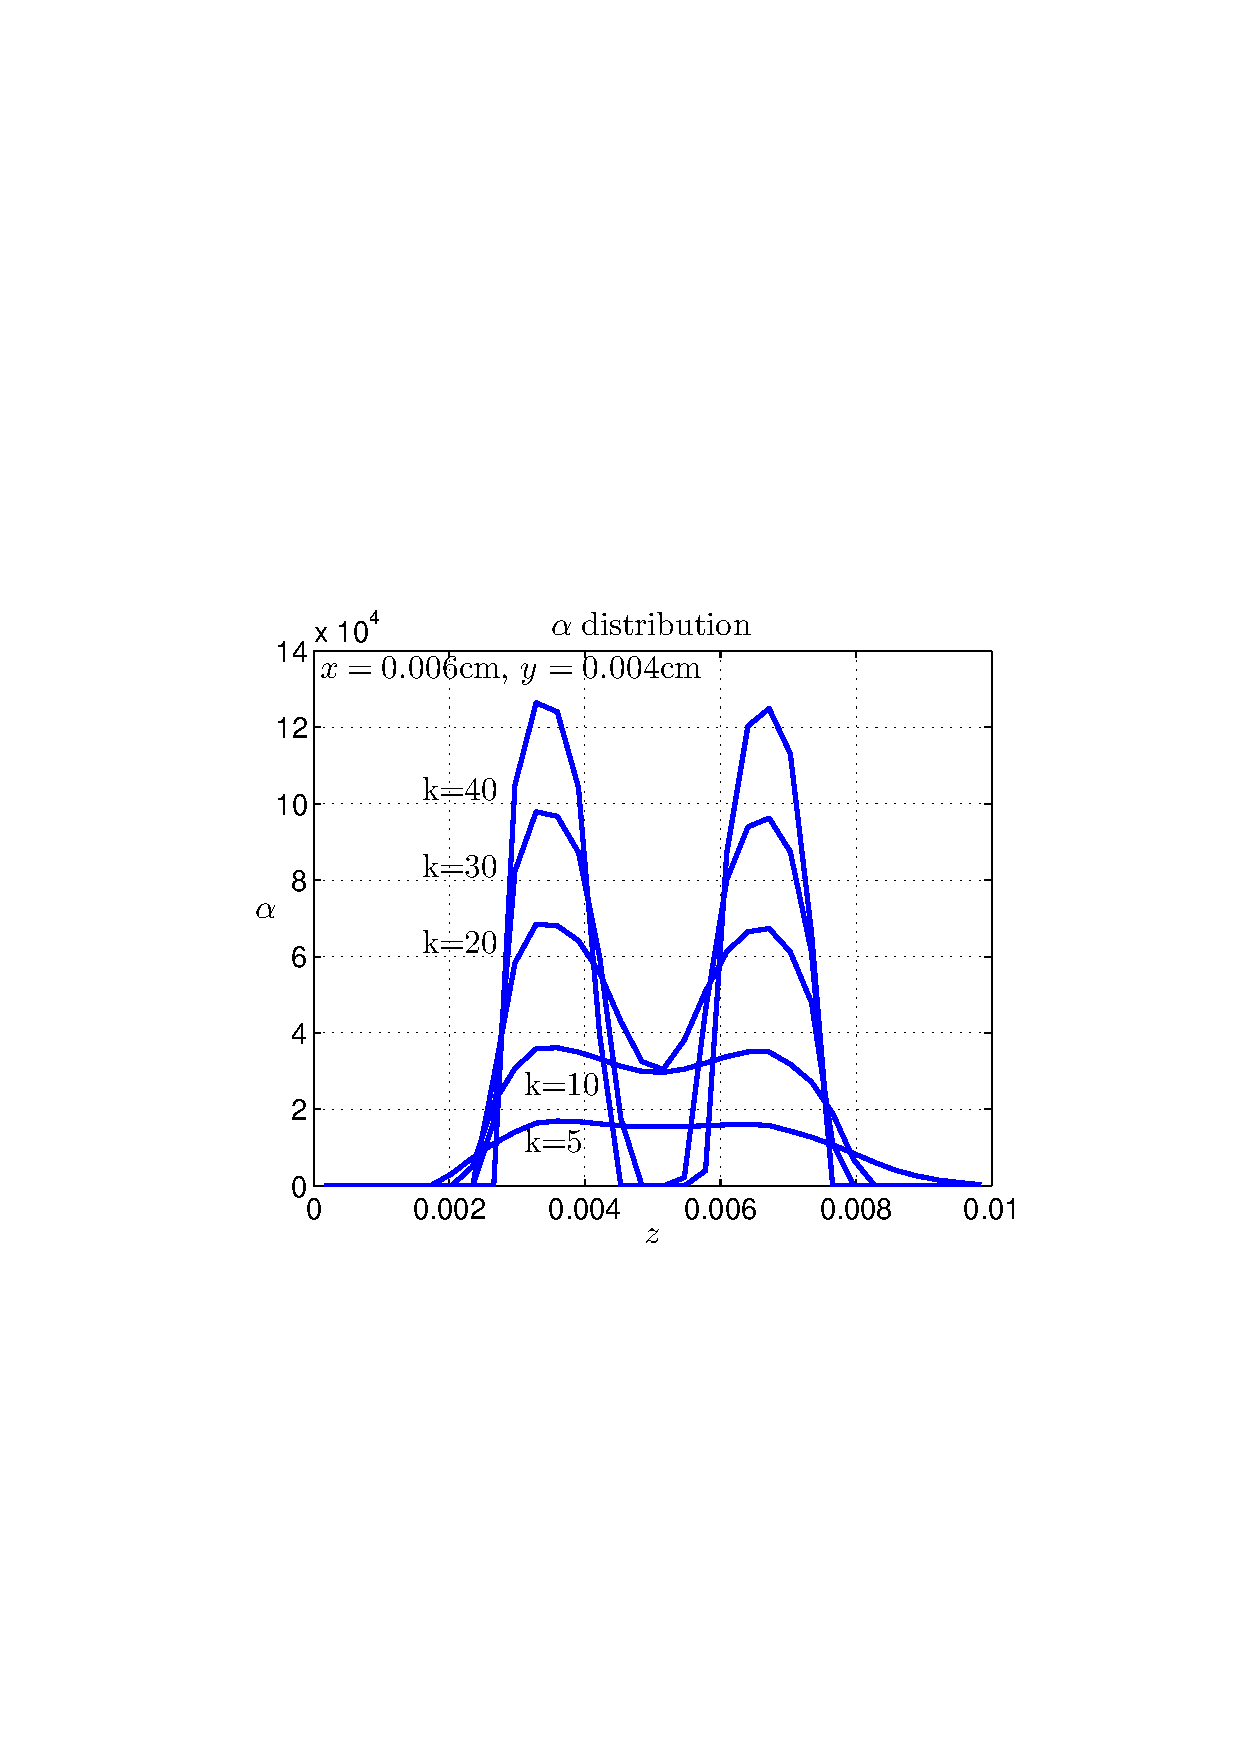
\includegraphics{example1alphaevolve}}
%    }
%  \end{figure}
%\end{example}


%%%%%%%%%%%%%%%%%%%%%%%%%%%%%%%%%%%%%%%%%%%%%%%%%%%%%%%%%%%%%%%%%%%%%%%%%
%\newpage
%\begin{example}{\bfseries Rototate the flow for $45$ degrees}
%%%%%%%%%%%%%%%%%%%%%%%%%%%%%%%%%%%%%%%%%%%%%%%%%%%%%%%%%%%%%%%%%%%%%%%%%
%%%%%%%%%%%%%%%%%%%%%%%%%%%%%%%%%%%%%%%%%%%%%%%%%%%%%%%%%%%%%%%%%%%%%%%%%
%\begin{tabular}{lr}
% \begin{minipage}[b]{12cm}
%\vspace{0.5cm}
%$S(y,z;y_c,z_c,\theta): (y,z)\mapsto (y_e,z_e)$, and
%  \begin{eqnarray*}
%  \\[-2cm]
%     y_e &= y_c + r \cos(\alpha+\theta) \\
%     z_e &= z_c + r \sin(\alpha+\theta)
%  \end{eqnarray*} 

%where $(r,\alpha)=\text{polar}(y,z)$
 
%Objective:
 %a flow map to rotate the flow 45 degrees centered at $(0.5,0.5)$ per period of the channel.
%\vspace{0cm}
%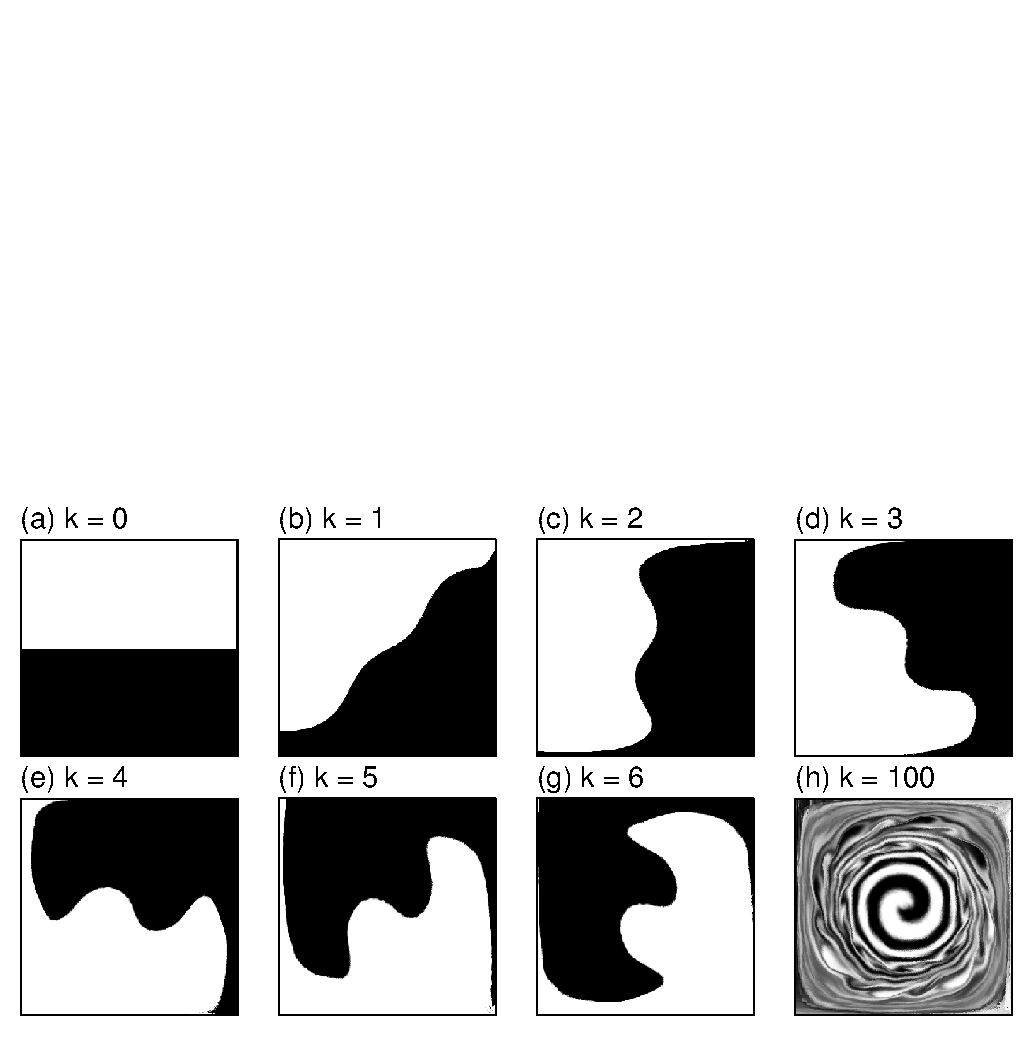
\includegraphics[width=1\textwidth,trim=0cm 0cm 0cm 8cm,clip]{example3simu}
% \end{minipage}
% & \begin{minipage}[b]{10cm}
%      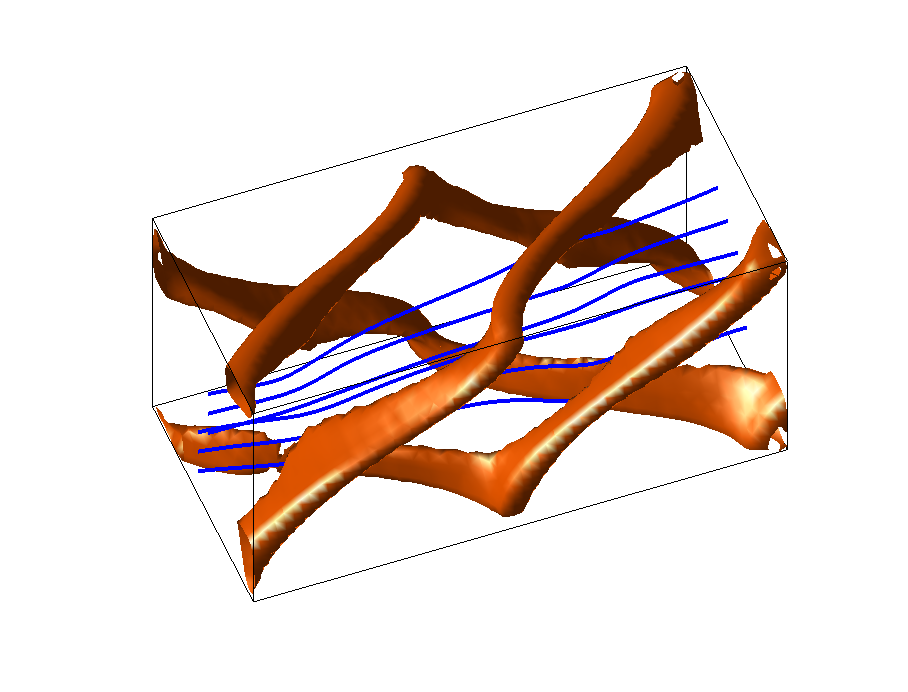
\includegraphics[width=0.8\textwidth,trim=1cm 0cm 1cm 1cm,clip]{example3structure}
%      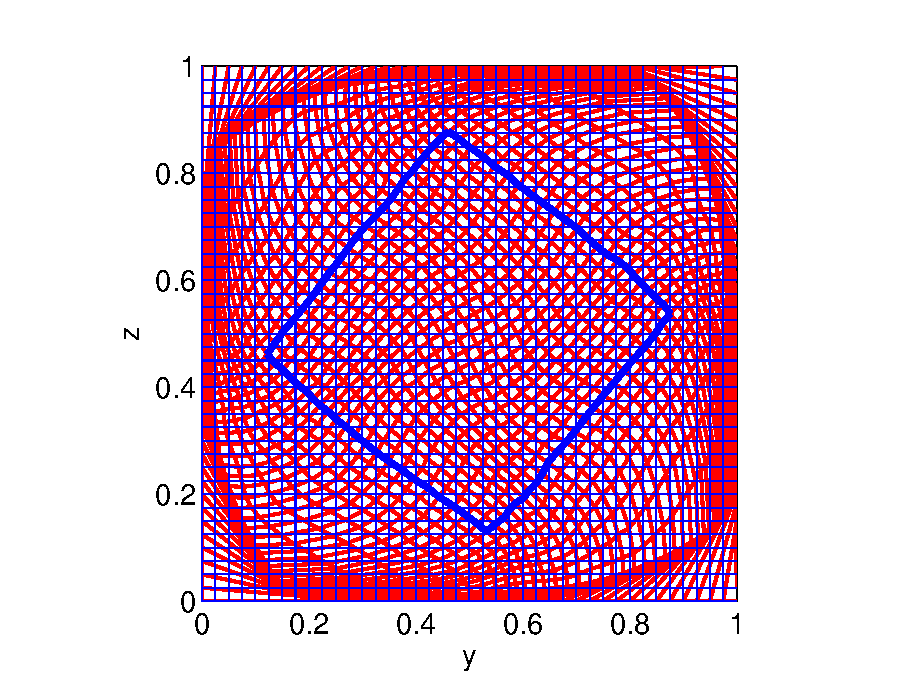
\includegraphics[width=0.8\textwidth,trim=1cm 1cm 1cm 1cm]{example3grid}
% \end{minipage}
%\end{tabular}
%\end{example}

%%%%%%%%%%%%%%%%%%%%%%%%%%%%%%%%%%%%%%%%%%%%%%%%%%%%%%%%%%%%%%%%%%%%%%%%%
\newpage
\oursection{Results}
%%%%%%%%%%%%%%%%%%%%%%%%%%%%%%%%%%%%%%%%%%%%%%%%%%%%%%%%%%%%%%%%%%%%%%%%%
%%%%%%%%%%%%%%%%%%%%%%%%%%%%%%%%%%%%%%%%%%%%%%%%%%%%%%%%%%%%%%%%%%%%%%%%%
%\begin{example}
  \begin{figure}
    \centerline{
       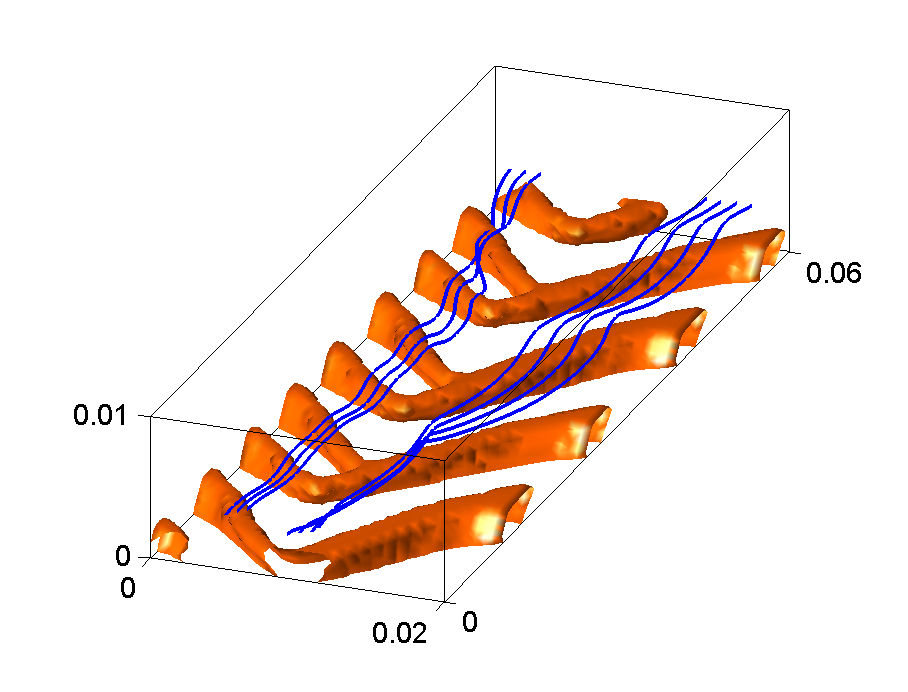
\includegraphics[width=0.45\textwidth,trim=1cm 0cm 0cm 0cm,clip]{myharringbonestructure}
       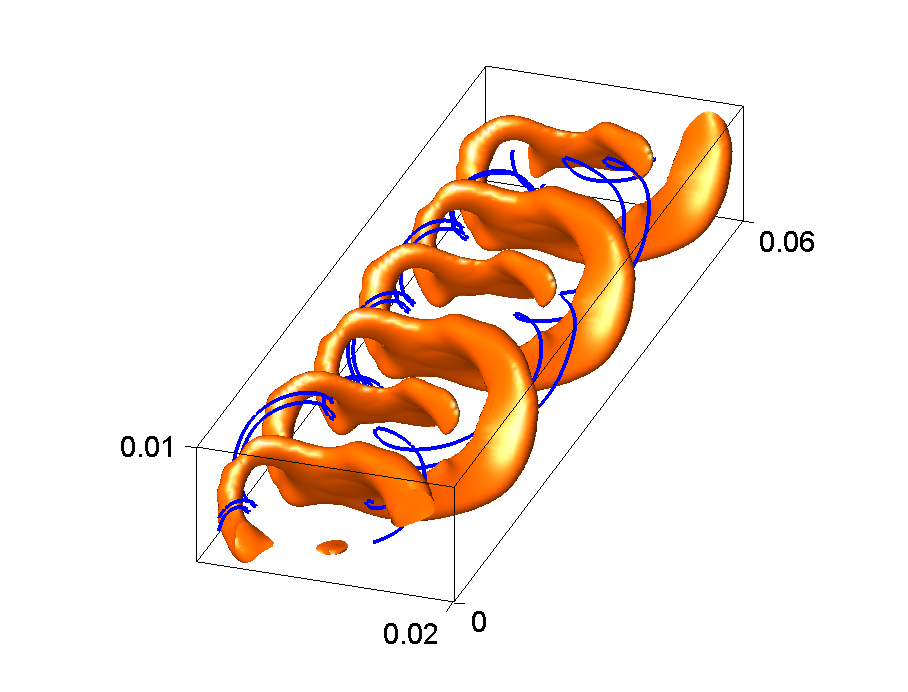
\includegraphics[width=0.45\textwidth,trim=1cm 0cm 1cm 0cm,clip]{my3dstructure}     
    }
  \end{figure}
\begin{itemize}\setlength{\parskip}{0pt}  \setlength{\itemsep}{10pt} \setlength{\topsep}{0pt}
\item Left: Optimal harryingbone-type channel.
\item Right: Optimal 3-D structured channel.  
\end{itemize}

%%%%%%%%%%%%%%%%%%%%%%%%%%%%%%%%%%%%%%%%%%%%%%%%%%%%%%%%%%%%%%%%%%%%%%%%%
%%%%%%%%%%%%%%%%%%%%%%%%%%%%%%%%%%%%%%%%%%%%%%%%%%%%%%%%%%%%%%%%%%%%%%%%%
\newpage
%%%%%%%%%%%%%%%%%%%%%%%%%%%%%%%%%%%%%%%%%%%%%%%%%%%%%%%%%%%%%%%%%%%%%%%%%
  \begin{figure}
    \centerline{
       \scalebox{0.65}[0.65]{\includegraphics{mixersimu}}
       \scalebox{0.65}[0.65]{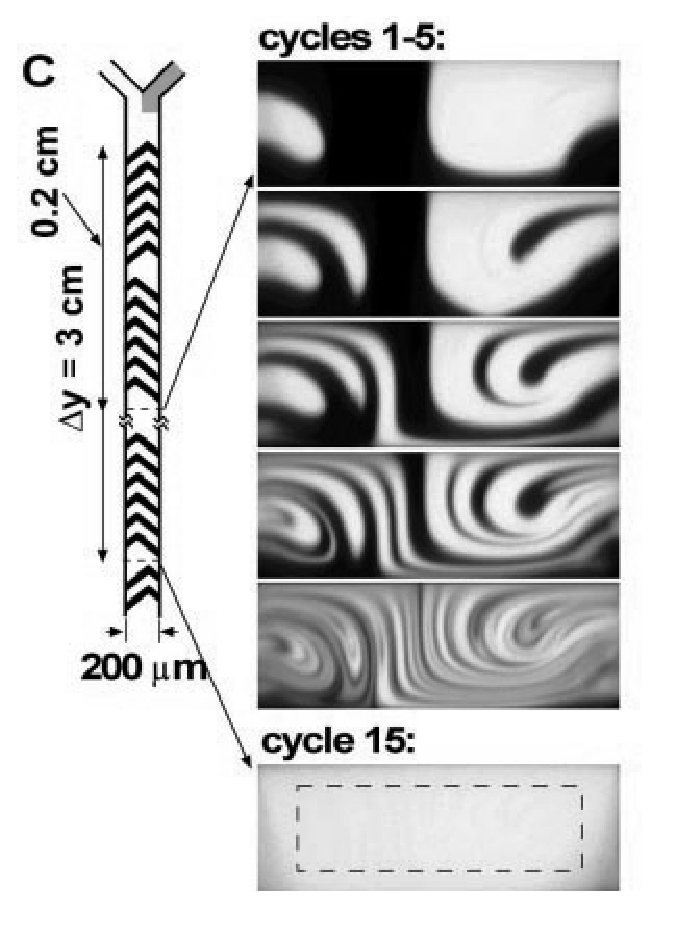
\includegraphics{stroockcrosssection0}}
    }
  \end{figure}
\vspace{-0.5cm}
\begin{figure}  
       \scalebox{0.60}[0.60]{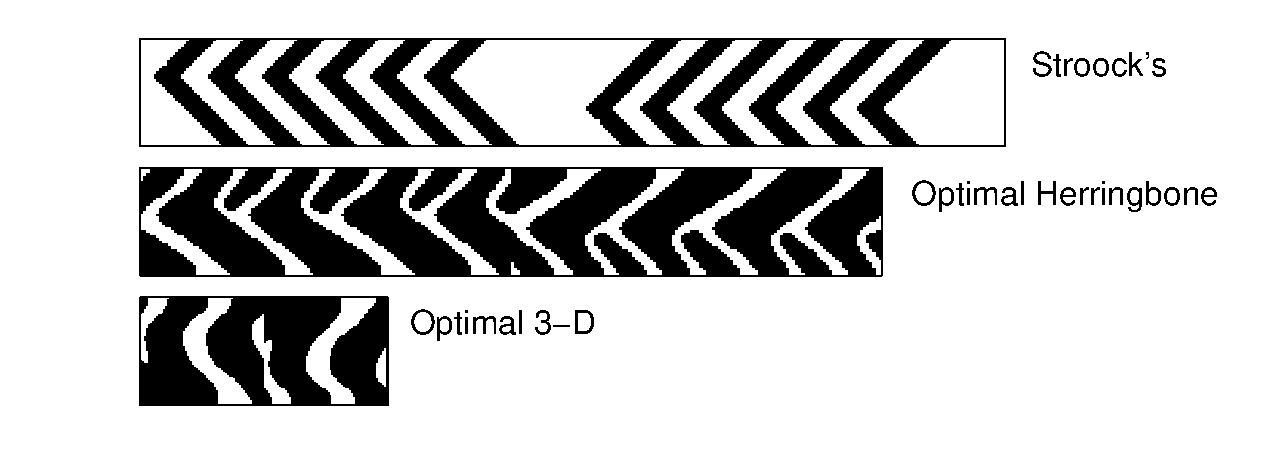
\includegraphics[trim=-2cm 0cm 0cm 0cm,clip]{example2fullcycle}}
\end{figure}  

%%%%%%%%%%%%%%%%%%%%%%%%%%%%%%%%%%%%%%%%%%%%%%%%%%%%%%%%%%%%%%%%%%%%%%%%%
%\newpage
%\oursection{Results}
%%%%%%%%%%%%%%%%%%%%%%%%%%%%%%%%%%%%%%%%%%%%%%%%%%%%%%%%%%%%%%%%%%%%%%%%%
%%%%%%%%%%%%%%%%%%%%%%%%%%%%%%%%%%%%%%%%%%%%%%%%%%%%%%%%%%%%%%%%%%%%%%%%%
% need two examples
%\begin{itemize}
%\item Cross-sections of the three channels.
%\end{itemize}
%  \begin{figure}
%    \centerline{
%       \scalebox{0.7}[0.7]{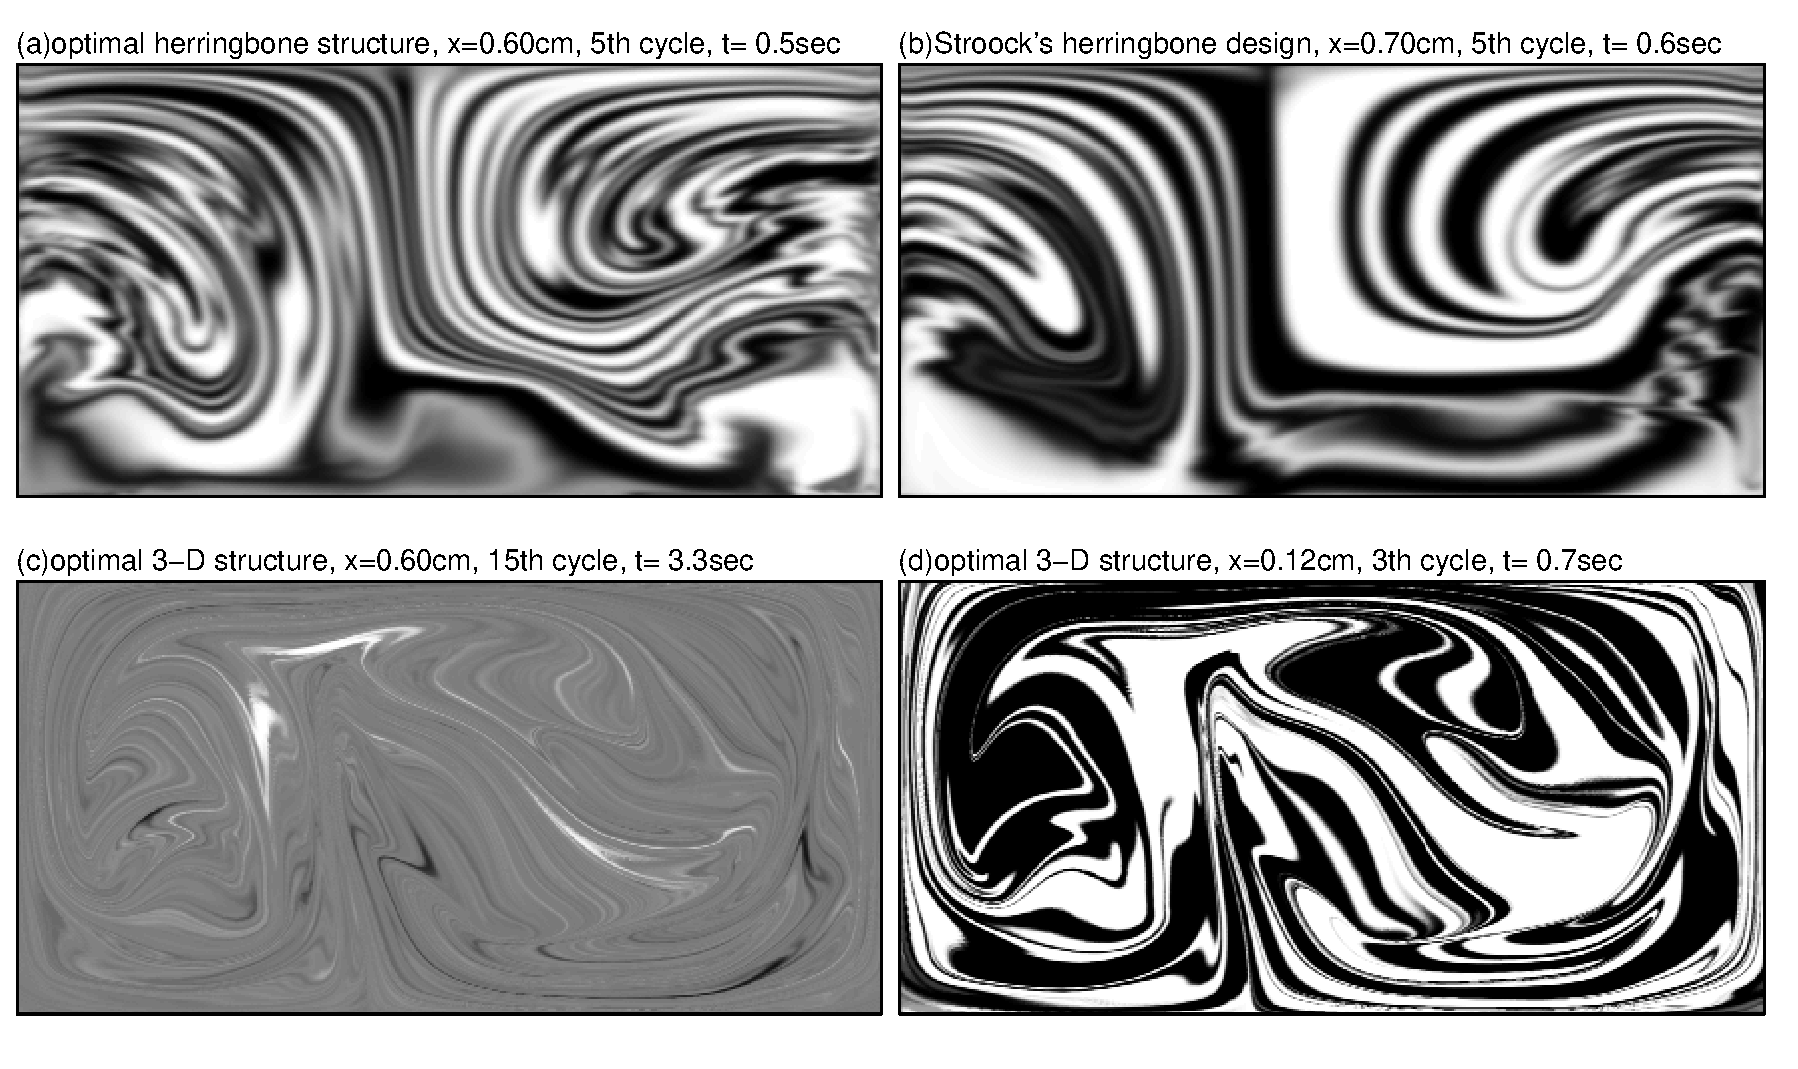
\includegraphics{example2crosscompare}}
%    }
%  \end{figure}
%%%%%%%%%%%%%%%%%%%%%%%%%%%%%%%%%%%%%%%%%%%%%%%%%%%%%%%%%%%%%%%%%%%%%%%%%
%%%%%%%%%%%%%%%%%%%%%%%%%%%%%%%%%%%%%%%%%%%%%%%%%%%%%%%%%%%%%%%%%%%%%%%%%
\newpage
\oursection{Results}
%%%%%%%%%%%%%%%%%%%%%%%%%%%%%%%%%%%%%%%%%%%%%%%%%%%%%%%%%%%%%%%%%%%%%%%%%

  \begin{figure}
    \centerline{
       \scalebox{0.6}[0.6]{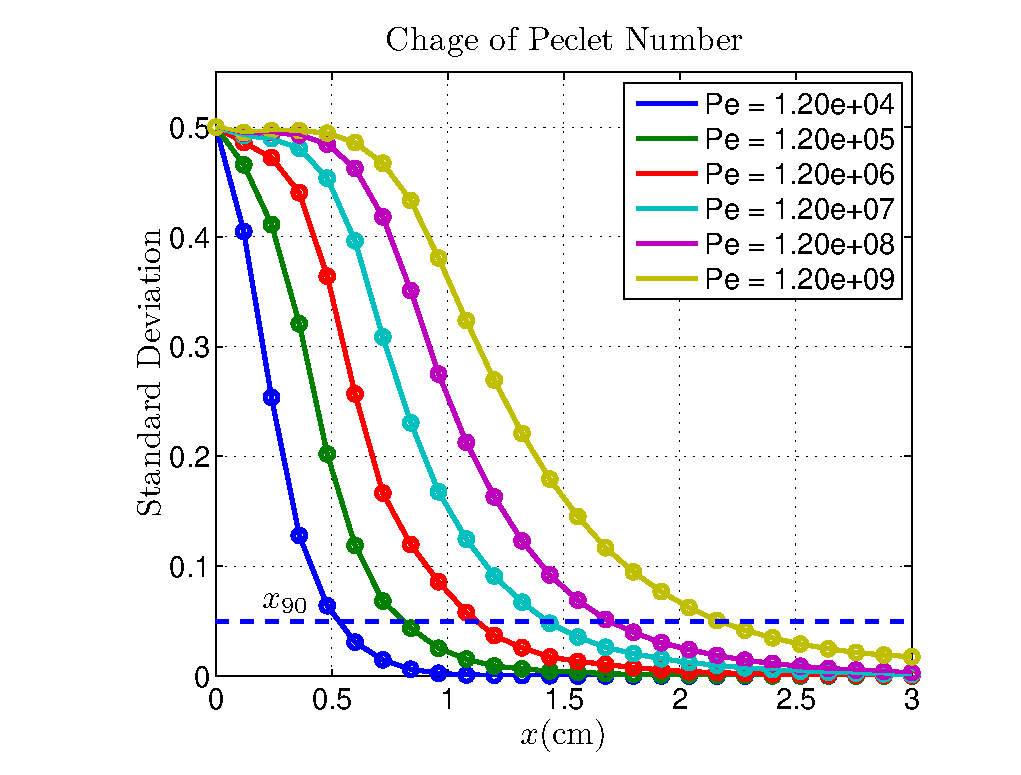
\includegraphics{example2veryPe2}}
       \scalebox{0.6}[0.6]{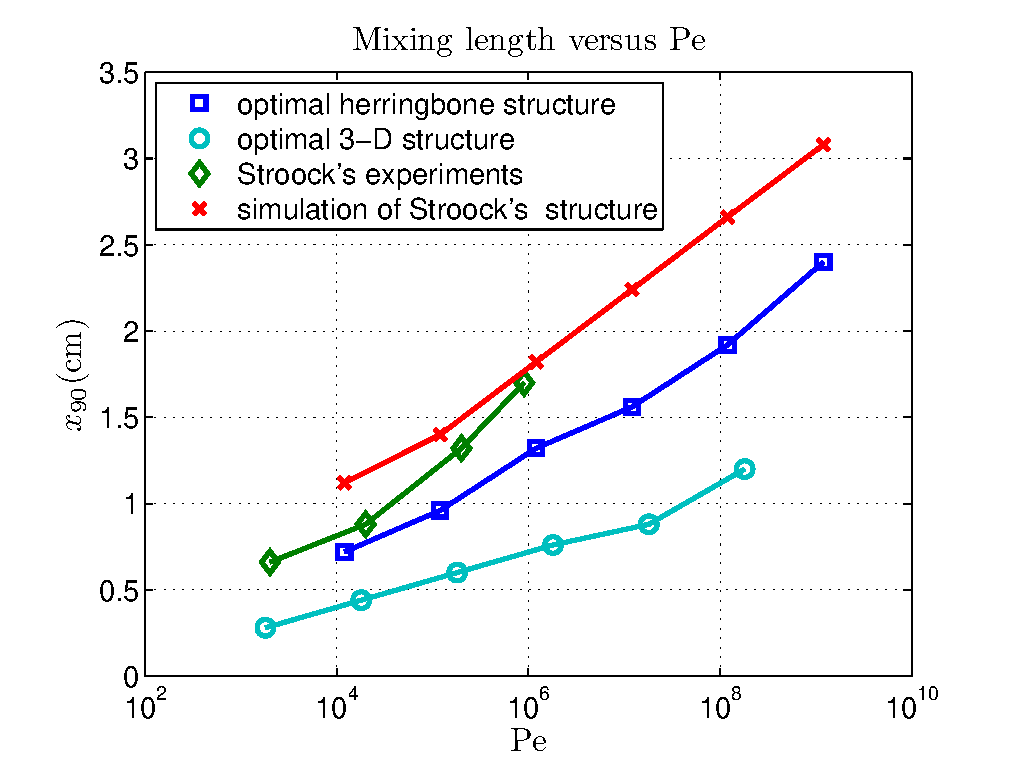
\includegraphics{example2mixinglength2}}
    }
  \end{figure}
%\end{example}
\begin{itemize}\setlength{\parskip}{0pt}  \setlength{\itemsep}{10pt} \setlength{\topsep}{0pt}
\item The mixing length($x_{90}$) is defined as the channel length required for the standard deviation of the color intensity dropping from $0.5$ to $0.05$. 
\item $x_{90}$ grows linearly with $\log(\text{Pe})$.
\end{itemize}


%%%%%%%%%%%%%%%%%%%%%%%%%%%%%%%%%%%%%%%%%%%%%%%%%%%%%%%%%%%%%%%%%%%%%%%%%
%%%%%%%%%%%%%%%%%%%%%%%%%%%%%%%%%%%%%%%%%%%%%%%%%%%%%%%%%%%%%%%%%%%%%%%%%
%\newpage
%\oursection{Results}
%%%%%%%%%%%%%%%%%%%%%%%%%%%%%%%%%%%%%%%%%%%%%%%%%%%%%%%%%%%%%%%%%%%%%%%%%
% \begin{figure}
%    \centerline{
%       \scalebox{0.7}[0.7]{\includegraphics{Stroockcrosssection}}
%       \scalebox{0.7}[0.7]{\includegraphics{stroockcrosssectionsimu}}
%    }
% \end{figure}
%
%%%%%%%%%%%%%%%%%%%%%%%%%%%%%%%%%%%%%%%%%%%%%%%%%%%%%%%%%%%%%%%%%%%%%%%%%
%%%%%%%%%%%%%%%%%%%%%%%%%%%%%%%%%%%%%%%%%%%%%%%%%%%%%%%%%%%%%%%%%%%%%%%%%
%\newpage
%\oursection{Results}
%%%%%%%%%%%%%%%%%%%%%%%%%%%%%%%%%%%%%%%%%%%%%%%%%%%%%%%%%%%%%%%%%%%%%%%%%


\newpage
\oursection{Conclusion}
%%%%%%%%%%%%%%%%%%%%%%%%%%%%%%%%%%%%%%%%%%%%%%%%%%%%%%%%%%%%%%%%%%%%%%%%%
%%%%%%%%%%%%%%%%%%%%%%%%%%%%%%%%%%%%%%%%%%%%%%%%%%%%%%%%%%%%%%%%%%%%%%%%%
\begin{itemize}
  \item We are successful in
    \begin{itemize}
       \item Building a gradient-based optimization scheme for microfluidic mixing channel design.
       \item Improving the current mixer. 
    \end{itemize}
  \item We fail in
    \begin{itemize}
       \item Linking the design parameters to ``mixing rate'' or ``mixing length''.
       \item Chaos needs to be designed.%Designing chaotic maps.
    \end{itemize}
  %\item A question about the mixing trajectories. 
\end{itemize}




\newpage
\oursection{Conclusion(For this talk)}
\begin{itemize}
\item ...
\end{itemize}

%%%%%%%%%%%%%%%%%%%%%%%%%%%%%%%%%%%%%%%%%%%%%%%%%%%%%%%%%%%%%%%%%%%%%%%%%%
\end{document}
